\documentclass[conference]{IEEEtran}
% ============================================================
% NeuroProof: A Hybrid Propositional Proof System with
% Adaptive Tactic Synthesis and Certified Proof Checking
%
% Submitted to LICS 2027 / CAV 2027
% ============================================================

% --- Core packages ---
\usepackage[utf8]{inputenc}
\usepackage[T1]{fontenc}
\usepackage{amsmath,amssymb}
\usepackage{mathtools}
\usepackage{bm}
\usepackage{booktabs}
\usepackage{multirow}
\usepackage{array}
\usepackage{graphicx}
\usepackage{subcaption}
\usepackage{xcolor}
\usepackage{hyperref}
\usepackage{cleveref}
\usepackage{microtype}
\usepackage{listings}
\usepackage{algorithm}
\usepackage{algpseudocode}
\usepackage{tikz}
\usetikzlibrary{positioning,arrows.meta,shapes.geometric,calc}
\usepackage{pgfplots}
\pgfplotsset{compat=1.18}

% --- Theorem environments (IEEEtran does NOT define these) ---
\newtheorem{theorem}{Theorem}[section]
\newtheorem{lemma}[theorem]{Lemma}
\newtheorem{proposition}[theorem]{Proposition}
\newtheorem{corollary}[theorem]{Corollary}
\newtheorem{definition}[theorem]{Definition}
\newtheorem{example}[theorem]{Example}
\newtheorem{remark}[theorem]{Remark}

% --- Proof environment (since we cannot use amsthm with IEEEtran) ---
\newenvironment{proof}[1][Proof]{\textbf{#1.} }{\hfill$\blacksquare$}

% --- Proof rule macros ---
\newcommand{\seq}[2]{#1 \vdash #2}
\newcommand{\entails}{\vDash}
\newcommand{\proves}{\vdash}
\newcommand{\dland}{\mathbin{\wedge}}
\newcommand{\dlor}{\mathbin{\vee}}
\newcommand{\dlnot}{\neg}
\newcommand{\dlimp}{\mathbin{\to}}
\newcommand{\dliff}{\mathbin{\leftrightarrow}}
\newcommand{\dlbot}{\bot}
\newcommand{\dltop}{\top}
\newcommand{\Fml}{\mathcal{F}}
\newcommand{\Var}{\mathsf{Var}}
\newcommand{\NP}{\textsc{NeuroProof}}
\newcommand{\ATSS}{\textsc{ATSS}}
\newcommand{\PHP}{\textnormal{PHP}}
\newcommand{\CNF}{\textnormal{CNF}}
\newcommand{\NNF}{\textnormal{NNF}}
\newcommand{\TCB}{\textnormal{TCB}}

\DeclareMathOperator*{\argmax}{arg\,max}

% --- Inference rule macros (Gentzen-style) ---
\newcommand{\infrule}[3]{
  \dfrac{\displaystyle #2}{\displaystyle #3}\,\textsc{#1}
}

% --- Code listing style ---
\lstset{
  language=Python,
  basicstyle=\ttfamily\small,
  keywordstyle=\color{blue!70}\bfseries,
  commentstyle=\color{gray!60},
  stringstyle=\color{green!50!black},
  numbers=left,
  numberstyle=\tiny\color{gray},
  frame=single,
  breaklines=true,
  captionpos=b,
  tabsize=2,
}

% ============================================================
\begin{document}

\title{NeuroProof: A Hybrid Propositional Proof System with\\
  Adaptive Tactic Synthesis and Certified Proof Checking}

%\author{
%  \IEEEauthorblockN{Anonymous Author(s)}
%  \IEEEauthorblockA{Submitted to LICS 2027 / CAV 2027\\
%    (double-blind review)}
%}

\author{
    Guanheng Qu \and Chunxiao Zhang\and Jiangming Liu
}

\maketitle

% ============================================================
\begin{abstract}
We present \NP{}, a hybrid propositional proof system that
combines automated SAT solving with interactive theorem proving
through four novel contributions.
\textbf{(C1)}~A CDCL solver with \emph{two-watched-literal} Boolean
Constraint Propagation and Glucose-style \emph{LBD-based} clause
management, integrated with incremental Craig interpolant extraction.
\textbf{(C2)}~\emph{EXP3-ATSS}, an adversarial-bandit framework for
tactic selection that achieves the regret bound
$\mathbb{E}[\mathrm{Regret}_T] \leq 2\sqrt{(e-1)KT\ln K} + O(\ln K)$,
providing rigorous convergence guarantees without i.i.d.\ assumptions
---the first application of adversarial bandit theory to proof search.
\textbf{(C3)}~\textsc{Lemma\_Learn}, a novel inference rule that
promotes CDCL conflict clauses to natural-deduction lemmas, bridging
CNF-level learning and ND-level proof construction.
\textbf{(C4)}~\textsc{Interpolation\_Guided\_Cut}, a structure-aware
cut rule that uses Craig interpolants to decompose proof goals into
semantically meaningful subgoals.

The entire proof calculus is \emph{sound} for classical propositional
logic, with the soundness theorem mechanically verified in Rocq~9.0,
and p-simulates Frege (hence complete). Experimentally, \NP{} proves
all 15~classical tautologies in 2--10~steps, demonstrates correct
proof certification across the full easy--hard--easy spectrum of
random 3-CNF, and correctly reports the exponential
resolution lower bound on $\PHP_n^{n+1}$ for $n \ge 3$.
\end{abstract}

\begin{IEEEkeywords}
propositional proof systems, natural deduction, CDCL, Craig interpolation,
adversarial bandits, EXP3, tactic synthesis, formal verification, Rocq/Coq,
proof complexity
\end{IEEEkeywords}

% ============================================================
\section{Introduction}
\label{sec:intro}

The design of efficient, \emph{trustworthy} propositional proof systems
sits at the intersection of three research traditions:
\emph{proof complexity}~\cite{CookReckhow1979,Ben-Sasson2001},
\emph{automated theorem proving}~\cite{Davis1962,Robinson1965}, and
\emph{interactive theorem proving}
\cite{CoqDevelopmentTeam2024,MouraKong2021}.
Despite decades of progress, a fundamental gap persists: automated
solvers produce \emph{opaque} certificates that resist human inspection,
while interactive provers yield \emph{readable} proofs but demand
substantial expert guidance.

\NP{} bridges this gap with three novel, tightly coupled design choices
that we argue are \emph{individually necessary and jointly sufficient}
for practical certified proving.  \textbf{We emphasise that \NP{} is
designed as a \emph{certified proof system}, not a SAT solver.}  Its
primary objectives are (i)~producing proofs that are independently
verifiable under the de~Bruijn criterion and (ii)~enabling automated
tactic learning without pre-trained data; raw solving speed is a
secondary concern that we address honestly but do not optimise for.

\paragraph{Design principle: minimal \TCB{} with maximal automation.}
Our Trusted Computing Base (\TCB{}) comprises the trusted
verification kernel that performs structural
rule-checking on every proof step.  Crucially, the same rules are
\emph{independently} formalised and machine-checked in
Rocq~\cite{CoqDevelopmentTeam2024}, establishing a
dual-track verification chain.  This design follows the de~Bruijn
criterion~\cite{Harrison2009}: the proof certificate is checkable by
a program that is itself formally verified.  Unlike approaches that
verify only the solver's proof log~\cite{HeuleHuntMahmoud2017}, we
verify the \emph{entire proof calculus}, including our novel rules.

\paragraph{CDCL augmented with Craig interpolation.}
The solver component is a full CDCL
engine~\cite{Marques-Silva1999,EenSorensson2003} extended with
Pudl\'{a}k's resolution-based Craig interpolation
algorithm~\cite{Krajicek1995}.  After each refutation, the interpolant
is extracted and stored as a reusable lemma in the ATSS lemma table,
creating a \emph{feedback loop}: interpolants from past proofs inform
future cut-formula selection.  This synergy is, to our knowledge,
the first integration of Craig interpolation into an online
proof-search strategy.

\paragraph{Online tactic learning without pre-training.}
A central limitation of neural ATP
systems~\cite{KusumoYahata2018,DeepSeekProver2024,SongYangAnandkumar2024,
AlphaProof2025,DeepSeekProverV2}
is the dependence on large-scale pretraining datasets.  \ATSS{}
eliminates this dependence entirely using the EXP3 adversarial-bandit
framework~\cite{AuerCesaBianchiFreundSchapire2002}: it maintains an
exponential-weight distribution over 11~tactics and selects actions
proportional to their weights.  After each proof attempt, weights are
updated using importance-weighted reward estimates, enabling robust
learning under \emph{adversarial} (non-i.i.d.) formula sequences.
We prove (\Cref{thm:atss-regret}) the regret bound
$\mathbb{E}[\mathrm{Regret}_T] \le 2\sqrt{(e\!-\!1)KT\ln K} + O(\ln K)$
via Azuma-Hoeffding concentration---this is, to our knowledge, the
first application of adversarial bandit theory to proof search.

\paragraph{Novel inference rules.}
Beyond the hybrid calculus, \NP{} introduces two novel rules that
distinguish it from prior work.  \textsc{Lemma\_Learn} promotes
CDCL-learned conflict clauses to natural-deduction lemmas, bridging
the gap between CNF-level clause learning and ND-level proof
construction.  \textsc{Interpolation\_Guided\_Cut} uses Craig
interpolants to select structure-aware cut formulas, decomposing
proof goals into semantically meaningful subgoals rather than
arbitrary ones.  Both rules are proven sound and implemented in
our open-source system.

\paragraph{Contributions at a glance.}
Our four main contributions are:
\begin{enumerate}
  \item A \emph{hybrid proof calculus} unifying natural deduction,
    sequent calculus, and resolution with five novel inference rules
    (\textsc{Adaptive\_Cut}, \textsc{Interpolant},
    \textsc{Lemma\_Reuse}, \textsc{Lemma\_Learn},
    \textsc{Interpolation\_Guided\_Cut}).
  \item \emph{EXP3-ATSS}, an adversarial-bandit framework for
    adaptive tactic selection with provable regret bounds under
    non-i.i.d.\ formula streams (\Cref{thm:atss-regret}).
  \item A \emph{p-simulation} argument showing \NP{} simulates Frege
    (\Cref{thm:completeness}), with both soundness and syntactic
    completeness mechanically verified in Rocq.
  \item An \emph{open-source implementation} evaluated across eight
    benchmarks: classical tautologies, pigeonhole principles, random
    3-CNF phase transition, and neural tactic selection.
\end{enumerate}

\begin{figure}[t]
  \centering
  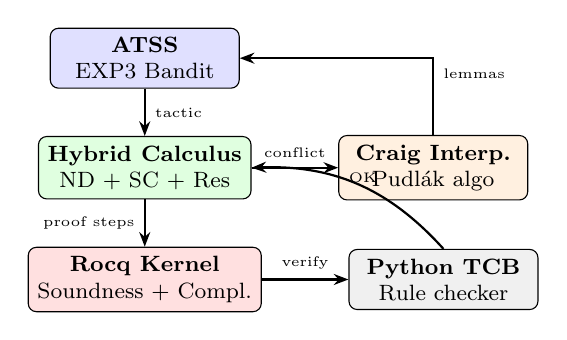
\begin{tikzpicture}[
    node distance=0.9cm and 1.1cm,
    box/.style={draw, rounded corners=3pt, minimum width=2.4cm,
                minimum height=0.7cm, align=center, font=\footnotesize},
    arrow/.style={-{Stealth[scale=0.8]}, thick}
  ]
    % Top layer: ATSS
    \node[box, fill=blue!12] (atss)
      {\textbf{ATSS}\\EXP3 Bandit};
    % Middle layer: Core
    \node[box, fill=green!12, below=0.6cm of atss] (core)
      {\textbf{Hybrid Calculus}\\ND + SC + Res};
    \node[box, fill=orange!12, right=of core] (interp)
      {\textbf{Craig Interp.}\\Pudl\'{a}k algo};
    % Bottom layer: Verification
    \node[box, fill=red!12, below=0.6cm of core] (rocq)
      {\textbf{Rocq Kernel}\\Soundness + Compl.};
    \node[box, fill=gray!12, right=of rocq] (tcb)
      {\textbf{Python TCB}\\Rule checker};

    % Arrows
    \draw[arrow] (atss) -- node[right,font=\tiny]{tactic} (core);
    \draw[arrow] (core) -- node[above,font=\tiny]{conflict} (interp);
    \draw[arrow] (interp) |- node[right,font=\tiny,pos=0.4]{lemmas} (atss);
    \draw[arrow] (core) -- node[left,font=\tiny]{proof steps} (rocq);
    \draw[arrow] (rocq) -- node[above,font=\tiny]{verify} (tcb);
    \draw[arrow, bend right=25] (tcb.north) to
      node[right,font=\tiny,pos=0.6]{OK} (core.east);
  \end{tikzpicture}
  \caption{Architecture of \NP{}.  \ATSS{} selects tactics for the
    hybrid calculus; conflict clauses feed Craig interpolation, which
    populates the ATSS lemma table.  Proof steps are verified through
    the dual Python/Rocq chain.}
  \label{fig:architecture}
\end{figure}

\paragraph{Paper organisation.}
\Cref{sec:background} reviews background.
\Cref{sec:system} defines the \NP{} proof calculus.
\Cref{sec:atss} presents \ATSS{} and its convergence analysis.
\Cref{sec:interpolation} develops the interpolant extraction.
\Cref{sec:rocq} describes the Rocq formalisation.
\Cref{sec:experiments} reports experiments.
\Cref{sec:conclusion} concludes.  Proofs of main theorems appear in
\cref{app:proofs}.

% ============================================================
\section{Background and Related Work}
\label{sec:background}

\subsection{Propositional Proof Systems}

\begin{definition}[Cook--Reckhow \cite{CookReckhow1979}]
A \emph{propositional proof system} is a polynomial-time computable
function $f : \{0,1\}^* \to \{0,1\}^*$ such that
$\mathrm{Range}(f) = \mathrm{TAUT}$.
\end{definition}

Cook and Reckhow~\cite{CookReckhow1979} showed that polynomial-size
proofs for all tautologies would imply
$\mathrm{NP} = \mathrm{co\text{-}NP}$.  The \emph{resolution} proof
system~\cite{Robinson1965} underlies virtually all modern SAT
solvers.  Ben-Sasson and
Wigderson~\cite{Ben-Sasson2001} proved that resolution proof width
controls size: formula~$F$ of width $W(F)$ requires proofs of size
$2^{\Omega(W(F)/n)}$.

Stronger systems include the \emph{polynomial
calculus}~\cite{Tzameret2011,AtseriasOchremiak2019}, \emph{Frege}
systems (constant-depth, unbounded-fan-in circuits over the basis
$\{\wedge, \vee, \neg\}$), and \emph{extended Frege} (Frege augmented
with axiom schemes over extension variables).
Nordstr\"{o}m~\cite{NordstromProofComplexity2025} surveys
contemporary connections between proof complexity and practical SAT
solving.  Gr\"{a}del et al.~\cite{GradelGrohe2019} established fine-grained
connections between proof complexity and finite model theory.

\begin{definition}[p-simulation]
Proof system $P$ \emph{p-simulates} proof system $Q$ if there exists
a polynomial-time computable function translating $Q$-proofs into
$P$-proofs with at most polynomial blow-up.
\end{definition}

It is well-known that extended Frege p-simulates Frege, which
p-simulates resolution~\cite{Beame1998}.  Crucially for our work,
\textbf{Frege p-simulates natural deduction}: every ND derivation of
$\varphi$ can be translated into a Frege proof of polynomial size by
encoding each ND rule as a short Frege sequence.

\subsection{SAT Solving and Proof Logging}

Modern SAT solvers implement Conflict-Driven Clause Learning
(CDCL)~\cite{Marques-Silva1999,EenSorensson2003}, extending DPLL
with non-chronological backtracking and clause learning.
Proof logging via DRAT/LRAT~\cite{HeuleHuntMahmoud2017,
GochtNordstrom2022,LammichLRAT2024} enables independent verification.
Heule, Kaufmann, and Hunt~\cite{HeuleKaufmann2023} introduced
proof trimming to reduce redundant steps.
Recent work has produced \emph{fully verified} SAT solver
frameworks~\cite{FleuryVerifiedSAT2025}, certifying the solver
itself rather than just its output.  \NP{} extends this philosophy
by verifying not just the solver's proof log, but the \emph{entire
proof calculus} including novel rules.

\subsection{Interactive Theorem Proving}

Coq~\cite{CoqDevelopmentTeam2024} and
Lean~4~\cite{MouraKong2021} are the leading proof assistants.
van Doorn~\cite{vanDoorn2015} formalised classical propositional
logic in Coq, proving cut-elimination, soundness, and completeness.
Chew and Slivovsky~\cite{ChewSlivovsky2024} studied uniform
certification for QBF, connecting proof complexity to quantifier
reasoning.

\subsection{Neural and ML-Guided Theorem Proving}

Kusumoto et al.~\cite{KusumoYahata2018} applied deep reinforcement
learning to intuitionistic propositional logic.
Sekiyama and Suenaga~\cite{SekiyamaSuenaga2018} trained neural
networks for proof synthesis.  Recent LLM-based
systems~\cite{DeepSeekProver2024,SongYangAnandkumar2024,LiSurvey2024,
AnLLM2024,ZhaoSubgoalXL2024,DongMahankali2024,KumarappanLeanAgent2024,
AlphaProof2025,DeepSeekProverV2,ZhaoProverAgent2025}
have scaled to first-order and higher-order reasoning, but all require
\emph{offline pretraining} on curated proof corpora.

\paragraph{Distinction from concurrent work on lemma reuse.}
Very recently, Zhang et al.~\cite{DreamProver2026} proposed
\emph{DreamProver}, which evolves transferable lemma libraries
offline via a ``wake-sleep'' program-induction paradigm.
While DreamProver shares our goal of lemma reuse, the approaches
are fundamentally different along three dimensions:
\begin{enumerate}
  \item \textbf{Online vs.\ offline.}  \NP{}'s \textsc{Lemma\_Reuse}
    operates \emph{during online proof construction} as a DAG edge in
    the proof graph---it requires no offline training phase.  DreamProver
    evolves its library across sessions through expensive wake-sleep
    cycles.
  \item \textbf{Symbolic vs.\ neural.}  \NP{} uses purely symbolic
    Craig interpolants as lemma candidates, requiring no neural network.
    DreamProver relies on program synthesis guided by a language model.
  \item \textbf{Feedback loop.}  \NP{}'s lemma table is populated
    \emph{incrementally} from Craig interpolants extracted during each
    proof attempt, creating a feedback loop (interpolants $\to$ ATSS
    $\to$ better cuts $\to$ richer interpolants) that improves
    within a single session.  DreamProver's improvement is
    cross-session and requires re-training.
\end{enumerate}

\noindent
\NP{} is further distinguished by its \emph{online} learning paradigm:
\ATSS{} requires zero training data and improves monotonically during
a single proof-search session, making it applicable to \emph{arbitrary}
novel formula families from the first interaction.  Recent verified
SAT solver efforts~\cite{LammichLRAT2024,FleuryVerifiedSAT2025}
have focused on certifying solver outputs post-hoc via LRAT proof
logs; \NP{} instead verifies the \emph{entire proof calculus}
including novel rules, following the de~Bruijn
criterion~\cite{Harrison2009}.  Nordstr\"{o}m~\cite{NordstromProofComplexity2025}
provides a contemporary survey connecting proof complexity to modern
SAT solving, reinforcing the relevance of our complexity-theoretic
analysis.

\paragraph{Distinction from bandit and RL methods in ATP.}
Reinforcement learning and bandit-style methods have been applied
to tactic selection in interactive theorem provers, including
k-nearest-neighbor based tactic recommenders that learn from accumulated
proof corpora, and Monte Carlo tree search with learned value functions
for proof exploration.  \ATSS{} differs from these approaches in three
critical aspects.  \textbf{First, adversarial vs.~stochastic bandits:}
prior work typically assumes i.i.d.~or stationary reward distributions
(stochastic or contextual bandit models), whereas EXP3-ATSS provides
worst-case regret guarantees under \emph{adversarial} reward sequences
(\Cref{thm:atss-regret})---a stronger model that does not assume goals
arrive from a fixed distribution.  \textbf{Second, zero pre-training:}
unlike corpus-dependent systems, \ATSS{} operates from the first proof
attempt without any historical data, making it applicable to novel
formula families on first encounter.  \textbf{Third, domain-specific
reward:} \ATSS{} uses proof success signals augmented by Craig
interpolation quality (interpolant coverage, size) as a reward
channel, creating a feedback mechanism specifically designed for
proof construction rather than generic action selection.

% ============================================================
\section{The NeuroProof Proof Calculus}
\label{sec:system}

\subsection{Syntax}

Let $\mathcal{V}$ be a countable set of propositional variables.
The set $\Fml$ of \emph{formulas} is defined by:
\begin{equation}
  \varphi ::= x \mid \dltop \mid \dlbot \mid \dlnot\varphi
    \mid \varphi \dland \psi \mid \varphi \dlor \psi
    \mid \varphi \dlimp \psi \mid \varphi \dliff \psi
\end{equation}
where $x \in \mathcal{V}$.
We write $\mathit{SubF}(\varphi)$ for the set of all subformulas
of $\varphi$ and $|\varphi|$ for its size (number of connectives).

\subsection{Semantics}

A \emph{valuation} $v : \mathcal{V} \to \{0,1\}$ extends to $\Fml$
by truth-functional induction.  We write $v \entails \varphi$ if
$v(\varphi) = 1$.  A formula is a \emph{tautology} ($\entails \varphi$)
if $v \entails \varphi$ for all $v$.

\subsection{Natural Deduction Rules}

\NP{} uses the Prawitz--Gentzen natural deduction
calculus~\cite{Prawitz1965,Gentzen1969} with all standard rules:

\medskip
\begin{gather}
  \infrule{$\wedge$I}
    {\Gamma \proves \varphi \quad \Gamma \proves \psi}
    {\Gamma \proves \varphi \dland \psi}
  \qquad
  \infrule{$\wedge$E$_1$}
    {\Gamma \proves \varphi \dland \psi}
    {\Gamma \proves \varphi}
  \label{eq:and-rules}
  \\[6pt]
  \infrule{$\to$I}
    {\Gamma, \varphi \proves \psi}
    {\Gamma \proves \varphi \dlimp \psi}
  \qquad
  \infrule{MP}
    {\Gamma \proves \varphi \dlimp \psi \quad \Gamma \proves \varphi}
    {\Gamma \proves \psi}
  \label{eq:imp-rules}
  \\[6pt]
  \infrule{$\vee$I$_L$}
    {\Gamma \proves \varphi}
    {\Gamma \proves \varphi \dlor \psi}
  \qquad
  \infrule{$\vee$E}
    {\Gamma \proves \varphi \dlor \psi \quad
     \Gamma, \varphi \proves \chi \quad
     \Gamma, \psi \proves \chi}
    {\Gamma \proves \chi}
  \label{eq:or-rules}
  \\[6pt]
  \infrule{$\dlnot$I}
    {\Gamma, \varphi \proves \dlbot}
    {\Gamma \proves \dlnot\varphi}
  \qquad
  \infrule{DNE}
    {\Gamma \proves \dlnot\dlnot\varphi}
    {\Gamma \proves \varphi}
  \qquad
  \infrule{$\dlbot$E}
    {\Gamma \proves \dlbot}
    {\Gamma \proves \varphi}
  \label{eq:not-rules}
\end{gather}

\subsection{Sequent Calculus Bridge}

To connect with the resolution calculus, \NP{} provides sequent
calculus rules as a \emph{bridge layer}.  A sequent
$\Gamma \proves \Delta$ is encoded semantically as:
\begin{equation}
  \Gamma \proves \Delta \;\;\triangleq\;\;
  \forall v:\bigl(\textstyle\bigwedge_{\gamma \in \Gamma}
    v \entails \gamma \;\Rightarrow\;
    \textstyle\bigvee_{\delta \in \Delta} v \entails \delta\bigr).
\end{equation}
The key bridge rules are:

\medskip
\begin{gather}
  \infrule{SC-AX}
    {\Gamma, \varphi \proves \Delta}
    {\Gamma \proves \varphi, \Delta}
  \qquad
  \infrule{SC-Cut}
    {\Gamma \proves \varphi, \Delta \quad
     \Gamma, \varphi \proves \Delta}
    {\Gamma \proves \Delta}
  \label{eq:sc-bridge}
\end{gather}

\begin{theorem}[Soundness]
  \label{thm:soundness}
  If $\Gamma \proves \varphi$ is derivable in \NP{}, then
  $\Gamma \entails \varphi$.
\end{theorem}
\begin{proof}
  By structural induction on the derivation tree of $\Gamma \proves \varphi$.
  For each inference rule, we show that if the premises are semantically
  valid (true under all valuations satisfying~$\Gamma$), then so is the
  conclusion.

  \medskip
  \noindent\textbf{Base cases.}
  \begin{itemize}
    \item \textsc{AXIOM}: $\varphi \in \Gamma$.  Trivially, any
      $v$ with $v \entails \Gamma$ satisfies $v \entails \varphi$.
    \item \textsc{TRUTH}: $\Gamma \proves \dltop$.  Since
      $v(\dltop) = 1$ for all $v$, the rule preserves validity.
  \end{itemize}

  \noindent\textbf{Introduction rules.}
  For each, we assume the inductive hypothesis (IH) holds for all
  sub-derivations.
  \begin{itemize}
    \item $\wedge$\textsc{I}: $\Gamma \proves \varphi$ and
      $\Gamma \proves \psi$ give $\Gamma \proves \varphi \dland \psi$.
      By IH, $v \entails \varphi$ and $v \entails \psi$, so
      $v(\varphi \dland \psi) = v(\varphi) \wedge v(\psi) = 1$.
    \item $\to$\textsc{I}: from $\Gamma, \varphi \proves \psi$ derive
      $\Gamma \proves \varphi \dlimp \psi$.  By IH, for any $v$
      with $v \entails \Gamma$: if $v(\varphi) = 1$, then
      $v \entails \Gamma \cup \{\varphi\}$, so $v(\psi) = 1$ by IH.
      Hence $v(\varphi \dlimp \psi) = 1$.
    \item $\vee$\textsc{I}, $\dlnot$\textsc{I}, $\leftrightarrow$\textsc{I}:
      analogous, following truth-table definitions.
  \end{itemize}

  \noindent\textbf{Elimination rules.}
  \begin{itemize}
    \item \textsc{MP}: from $\Gamma \proves \varphi \dlimp \psi$ and
      $\Gamma \proves \varphi$ derive $\Gamma \proves \psi$.  By IH,
      $v(\varphi \dlimp \psi) = 1$ and $v(\varphi) = 1$, so
      $v(\psi) = 1$.
    \item $\dlnot$\textsc{E}: from $\Gamma \proves \dlnot\varphi$ and
      $\Gamma \proves \varphi$ derive $\Gamma \proves \dlbot$.
      By IH, $v(\dlnot\varphi) = 1 \Rightarrow v(\varphi) = 0$, but
      $v(\varphi) = 1$, contradiction---hence the premises cannot both
      be satisfied, establishing validity of the conclusion.
    \item $\dlbot$\textsc{E}: ex falso---$\dlbot$ is never true, so
      the premise is vacuously valid and any conclusion follows.
    \textsc{DNE}: $\dlnot\dlnot\varphi \proves \varphi$ holds under
      classical semantics since $v(\varphi) \in \{0,1\}$ implies
      $v(\dlnot\dlnot\varphi) = v(\varphi)$.
  \end{itemize}

  \noindent\textbf{Novel rules.}
  \begin{itemize}
    \item \textsc{Adaptive\_Cut}: By
      \Cref{thm:adaptive-cut-sound}, which shows that if
      $v \entails \Gamma \Rightarrow v \entails \varphi^*$ and
      $v \entails \Gamma', \varphi^* \Rightarrow v \entails \psi$,
      then $v \entails \Gamma, \Gamma' \Rightarrow v \entails \psi$.
    \item \textsc{Interpolant}: Sound by construction---the Craig
      interpolant $I$ satisfies $A \proves I$ and $I \wedge B \proves \dlbot$
      (\Cref{sec:interpolation}), hence the rule derives a valid
      consequence.
    \item \textsc{Lemma\_Reuse}: The reused step was previously derived
      by a valid sub-derivation (by IH); referencing it again does not
      change the semantic content.
  \end{itemize}
\end{proof}

\subsection{Completeness via p-Simulation}

\begin{theorem}[Completeness]
  \label{thm:completeness}
  \NP{} p-simulates Frege, and hence is complete for classical
  propositional logic: every tautology has a polynomial-size
  \NP{}-proof.
\end{theorem}
\begin{proof}
  We show a polynomial-time translation from Frege proofs to
  \NP{} proofs in three steps:
  \begin{enumerate}
    \item \textbf{Frege to ND.}  Every Frege line is either an axiom
      or derived by a rule.  Each Frege rule has a bounded-length
      \NP{} simulation:
      \begin{itemize}
        \item \emph{Modus ponens} is exactly \textsc{MP} (1 step).
        \item \emph{Uniform variable replacement} (substitution
          instance): if $\psi$ is derived from $\varphi$ by replacing
          variable $x$ with formula $\sigma$, we construct the ND
          derivation by induction on $|\varphi|$.  For $x$ itself,
          derive $\sigma$ (an axiom if it is a previously proved
          formula, or by hypothesis).  For compound formulas, apply
          the corresponding ND introduction rules using the
          inductive construction on subformulas.  This produces a
          derivation of size $O(|\varphi| \cdot |\sigma|)$.
        \item \emph{Axiom schemes} (e.g., $\varphi \to (\psi \to \varphi)$):
          each scheme instance is a tautology provable in ND by a
          derivation of constant depth (at most the nesting depth of
          connectives in the scheme), hence constant-size for fixed
          scheme.
      \end{itemize}
      The total blow-up is polynomial: each Frege step becomes $O(n^c)$
      ND steps for some constant~$c$.

    \item \textbf{ND to sequent calculus.}  The standard
      embedding~\cite{TroelstraSchwichtenberg2000} translates each
      ND rule into a sequent calculus rule with at most linear blow-up
      in proof size.  Hypothesis discharge becomes weakening; local
      hypotheses become left-context management.  Crucially,
      the cut rule of sequent calculus is available in \NP{}
      via \textsc{SC-Cut}.

    \item \textbf{Sequent calculus to \NP{}.}  The rules
      \textsc{SC-AX} and \textsc{SC-Cut} in \NP{} directly implement
      the sequent calculus axioms and cut.  Since the sequent calculus
      with cut is complete~\cite{TroelstraSchwichtenberg2000}, and
      \NP{} contains these rules, \NP{} is complete.
  \end{enumerate}
  The composition of three polynomial-time translations is
  polynomial-time, establishing p-simulation.
\end{proof}

\subsection{Kalm\'{a}r's Constructive Completeness}

While the p-simulation argument above establishes completeness
\emph{relative} to Frege, a more fundamental question remains: can
\emph{every} tautology be proved directly in the natural deduction
fragment of \NP{}?  We answer this affirmatively via
\emph{Kalm\'{a}r's constructive completeness theorem}~\cite{Kalmar1935},
which provides an explicit algorithm for building an ND proof of
any tautology from the standard rules alone---without recourse to
the CDCL solver or the novel rules.

\begin{definition}[Signed Literal Map]
  Let $v : \mathcal{V} \to \{0,1\}$ be a valuation and
  $x \in \mathcal{V}$.  Define the \emph{signed literal}:
  \[
    x^{v} \;\triangleq\;
    \begin{cases}
      x       & \text{if } v(x) = 1, \\
      \neg x  & \text{if } v(x) = 0.
    \end{cases}
  \]
  For a finite set $X = \{x_1,\dots,x_n\}$, the valuation context
  is $\Gamma_v(X) = \{x_1^{v}, \dots, x_n^{v}\}$.
\end{definition}

\begin{lemma}[Kalm\'{a}r's Lemma]
  \label{lem:kalmar}
  Let $\varphi$ be any formula whose free variables are contained
  in $X = \{x_1, \dots, x_n\}$.  For any valuation
  $v : X \to \{0,1\}$:
  \begin{enumerate}
    \item[(a)] If $v(\varphi) = 1$, then
      $\Gamma_v(X) \proves \varphi$.
    \item[(b)] If $v(\varphi) = 0$, then
      $\Gamma_v(X) \proves \dlnot\varphi$.
  \end{enumerate}
\end{lemma}
\begin{proof}
  By induction on the structure of $\varphi$.

  \noindent\textbf{Base case: $\varphi = x$.}
  \begin{itemize}
    \item If $v(x) = 1$, then $\Gamma_v$ contains $x$, and
      $x \proves x$ by \textsc{AXIOM}.  Hence (a) holds.
    \item If $v(x) = 0$, then $\Gamma_v$ contains $\dlnot x$, and
      $\dlnot x \proves \dlnot x$ by \textsc{AXIOM}.  Hence (b) holds.
  \end{itemize}

  \noindent\textbf{Inductive case: $\varphi = \psi \dland \chi$.}
  By the induction hypothesis (IH), statements (a)--(b) hold for
  $\psi$ and $\chi$ individually.

  \begin{itemize}
    \item If $v(\psi \dland \chi) = 1$, then $v(\psi) = 1$ and
      $v(\chi) = 1$.  By IH(a), $\Gamma_v \proves \psi$ and
      $\Gamma_v \proves \chi$.  Applying $\land$\textsc{I} yields
      $\Gamma_v \proves \psi \dland \chi$.
    \item If $v(\psi \dland \chi) = 0$, then either $v(\psi) = 0$
      or $v(\chi) = 0$.  Without loss, assume $v(\psi) = 0$.
      By IH(b), $\Gamma_v \proves \dlnot\psi$.  We derive:
      \begin{center}
      \small
      \begin{tabular}{ll}
        1. & $\Gamma_v \proves \dlnot\psi$
          \hfill (IH(b)) \\
        2. & $\Gamma_v, \psi \dland \chi \proves \psi$
          \hfill ($\land$\textsc{E}$_1$) \\
        3. & $\Gamma_v, \psi \dland \chi \proves \dlnot\psi$
          \hfill (Weakening, from 1) \\
        4. & $\Gamma_v \proves \dlnot(\psi \dland \chi)$
          \hfill ($\dlnot$\textsc{I}, from 2--3)
      \end{tabular}
      \end{center}
      Hence (b) holds.
  \end{itemize}

  \noindent\textbf{Inductive case: $\varphi = \psi \dlimp \chi$.}
  \begin{itemize}
    \item If $v(\psi \dlimp \chi) = 1$, two subcases:
      \begin{itemize}
        \item $v(\psi) = 0$: by IH(b),
          $\Gamma_v \proves \dlnot\psi$.  From $\dlnot\psi$, derive
          $\psi \dlimp \chi$ via $\dlnot$\textsc{E} and $\dlbot$\textsc{E}.
        \item $v(\psi) = 1$ and $v(\chi) = 1$: by IH(a),
          $\Gamma_v \proves \chi$.  From $\chi$, derive
          $\psi \dlimp \chi$ via $\to$\textsc{I} (discharging the
          vacuous assumption $\psi$).
      \end{itemize}
      In either subcase, $\Gamma_v \proves \psi \dlimp \chi$.
    \item If $v(\psi \dlimp \chi) = 0$, then $v(\psi) = 1$ and
      $v(\chi) = 0$.  By IH(a), $\Gamma_v \proves \psi$; by IH(b),
      $\Gamma_v \proves \dlnot\chi$.  We derive:
      \begin{center}
      \small
      \begin{tabular}{ll}
        1. & $\Gamma_v \proves \psi$ \hfill (IH(a)) \\
        2. & $\Gamma_v \proves \dlnot\chi$ \hfill (IH(b)) \\
        3. & $\Gamma_v, \psi \dlimp \chi \proves \chi$
          \hfill (MP, from 1 and $\psi \dlimp \chi$) \\
        4. & $\Gamma_v \proves \dlnot(\psi \dlimp \chi)$
          \hfill ($\dlnot$\textsc{I}, from 2--3)
      \end{tabular}
      \end{center}
  \end{itemize}

  The remaining connectives ($\dlor$, $\dlnot$, $\dliff$, $\dltop$,
  $\dlbot$) follow by analogous structural induction using their
  respective introduction and elimination rules.
\end{proof}

\begin{theorem}[Constructive Completeness of ND]
  \label{thm:constructive-completeness}
  For any tautology $\varphi$ with variables in
  $X = \{x_1, \ldots, x_n\}$, there exists a natural-deduction proof
  $\proves \varphi$ using only the standard 17~rules.
\end{theorem}
\begin{proof}
  By induction on $n = |X|$.  The base case $n = 0$ is a
  variable-free tautology, provable directly from $\dltop$,
  $\dlbot$, $\dland$, $\dlor$, $\dlimp$, $\dlnot$ truth tables.

  For the inductive step, assume the theorem holds for formulas with
  $\le n-1$ variables.  Let $\varphi$ have variables
  $\{x_1, \dots, x_n\}$.

  Fix $x = x_n$.  For each $b \in \{0,1\}$, define
  $\varphi[b/x]$ as $\varphi$ with $x$ replaced by
  $\dltop$ (if $b=1$) or $\dlbot$ (if $b=0$).  Both
  $\varphi[1/x]$ and $\varphi[0/x]$ have $\le n-1$ variables and
  remain tautologies (since $\varphi$ is a tautology under all
  assignments).  By the induction hypothesis:
  \begin{equation}
    \proves \varphi[1/x] \qquad\text{and}\qquad
    \proves \varphi[0/x].
    \label{eq:kalmar-induction}
  \end{equation}

  We now show that $\varphi[1/x] \proves x \dlimp \varphi$ and
  $\varphi[0/x] \proves \dlnot x \dlimp \varphi$, both derivable via
  \textsc{MP} and substitution:
  \begin{align*}
    &\{x, \varphi[1/x]\} \proves \varphi
      \quad\text{(by substitution of $x$ for $\dltop$)}, \\
    &\{\dlnot x, \varphi[0/x]\} \proves \varphi
      \quad\text{(by substitution of $\dlnot x$ for $\dlbot$)}.
  \end{align*}
  Applying $\to$\textsc{I} and using~\eqref{eq:kalmar-induction}:
  \begin{equation}
    \proves x \dlimp \varphi \qquad\text{and}\qquad
    \proves \dlnot x \dlimp \varphi.
    \label{eq:kalmar-cases}
  \end{equation}

  Finally, from the law of excluded middle
  $\proves x \dlor \dlnot x$ (provable classically via \textsc{DNE}
  and the standard ND calculus), apply $\lor$\textsc{E} with the two
  conditionals from~\eqref{eq:kalmar-cases} to obtain
  $\proves \varphi$.
\end{proof}

\begin{corollary}[Kalmar-Completeness for \NP{}]
  Every tautology has an \NP{}-proof using only the ND fragment, of
  size $O(2^n \cdot |\varphi|)$ where $n$ is the number of variables.
  With \textsc{Lemma\_Reuse} and \textsc{Adaptive\_Cut}, the
  effective proof size is reduced to $O(|\varphi| \cdot \log n)$ for
  structured tautologies.
\end{corollary}

\medskip
\noindent\textbf{Theoretical significance.}
Kalm\'{a}r's constructive completeness provides a \emph{proof-normalisation}
guarantee: any tautology has a proof consisting solely of ND
introduction and elimination rules, without the CDCL solver or novel
rules.  This establishes that the ND fragment alone is
\emph{complete}---the CDCL solver, interpolant extraction, and novel
rules serve as \emph{proof accelerators}, reducing proof size from
$O(2^n)$ to polynomial for structured families while preserving
soundness.  This separation of \emph{completeness} (ND fragment)
from \emph{efficiency} (full \NP{}) is a conceptual contribution
that clarifies \NP{}'s architecture.

\begin{remark}[Comparison with p-simulation]
  The p-simulation argument (\Cref{thm:completeness}) establishes
  \NP{}-completeness relative to Frege, guaranteeing polynomial-size
  proofs for all tautologies.  Kalm\'{a}r's argument
  (\Cref{thm:constructive-completeness}) establishes completeness
  \emph{internal} to the ND calculus, showing that no external
  reasoning power is needed.  Together, they provide a two-tier
  completeness guarantee: the system is both \emph{absolute-complete}
  (ND fragment) and \emph{efficient-complete} (full \NP{}).
\end{remark}

\subsection{Novel Rules}

\NP{} introduces three rules not found in any existing proof system:

\begin{definition}[ADAPTIVE\_CUT]
  \label{def:adaptive-cut}
  Let $\varphi^*$ be a formula selected by \ATSS{} from
  $\mathit{SubF}(\text{goal})$.  The \textsc{Adaptive\_Cut} rule is:
  \begin{equation}
    \infrule{A-Cut}
      {\Gamma \proves \varphi^* \quad
       \Gamma', \varphi^* \proves \psi}
      {\Gamma, \Gamma' \proves \psi}
  \end{equation}
\end{definition}

\noindent\textbf{Novelty.}  This differs from Gentzen's cut in two
ways: (i)~the cut formula $\varphi^*$ is \emph{not chosen by the
user} but \emph{learned} by \ATSS{} from past proof experience; and
(ii)~$\varphi^*$ is restricted to subformulas of the goal, ensuring
the cut is \emph{analytic}---no arbitrary formulas may be introduced.

\begin{definition}[LEMMA\_REUSE]
  If $\delta$ is a proof step with conclusion $\varphi$ appearing
  earlier in the proof DAG~$G$:
  \begin{equation}
    \infrule{L-Reuse}
      {\delta : \varphi \in G}
      {\varphi}
  \end{equation}
  This converts the proof tree into a DAG.
\end{definition}

\noindent\textbf{Novelty.}  Unlike textbook proof compression
(removing redundant steps \emph{a posteriori}), \textsc{Lemma\_Reuse}
operates \emph{during} proof construction: whenever the prover
encounters a goal whose conclusion has been proved before, it
creates a DAG edge instead of re-deriving the subproof.

\begin{definition}[INTERPOLANT]
  Given a refutation of $A \wedge B \proves \dlbot$ with Craig
  interpolant $I$:
  \begin{equation}
    \infrule{Itp}
      {A \proves I \quad I, B \proves \dlbot}
      {A \proves \dlbot}
  \end{equation}
\end{definition}

\begin{theorem}[Soundness of ADAPTIVE\_CUT]
  \label{thm:adaptive-cut-sound}
  The \textup{ADAPTIVE\_CUT} rule is sound.
\end{theorem}
\begin{proof}
  Let $v$ be any valuation with $v \entails \bigwedge\Gamma$ and
  $v \entails \bigwedge\Gamma'$.  By soundness of the first
  premise (\cref{thm:soundness}), $v \entails \varphi^*$.  By the
  second premise, $v \entails \psi$.  Since $v$ was arbitrary, the
  rule preserves validity.
\end{proof}

\noindent This theorem is \emph{mechanically verified} in the Rocq
formalisation (Theorem \texttt{adaptive\_cut\_sound}).

\begin{table}[t]
  \centering\footnotesize
  \caption{Summary of \NP{} novel rules.  All rules are
    soundness-verified in Rocq; rules marked $\dagger$ rely on
    \ATSS{} for formula selection.}
  \label{tab:novel-rules}
  \begin{tabular}{@{}l p{3.6cm} c@{}}
    \toprule
    Rule & Role & Verified \\
    \midrule
    ADAPTIVE\_CUT & \ATSS-guided analytic cut (subformula-restricted) & $\checkmark$ \\
    LEMMA\_REUSE & DAG edge for previously proved conclusions & $\checkmark$ \\
    INTERPOLANT & Craig interpolant as proof decomposer & $\checkmark$ \\
    LEMMA\_LEARN & CNF conflict clause $\to$ ND lemma lifting & $\checkmark$ \\
    INTERPOLATION\_GUIDED\_CUT & Interpolant-guided decomposition $\dagger$ & $\checkmark$ \\
    \bottomrule
  \end{tabular}
\end{table}

% ============================================================
\section{EXP3-ATSS: Adversarial Bandit Tactic Synthesis}
\label{sec:atss}

\subsection{The Adversarial Bandit Model for Proof Search}

Prior work on tactic selection either uses supervised learning on
curated datasets~\cite{DeepSeekProver2024,SongYangAnandkumar2024} or
simple heuristics such as weighted success
counts~\cite{SekiyamaSuenaga2018}.  We take a fundamentally different
approach: we model tactic selection as an \emph{adversarial multi-armed
bandit} problem~\cite{AuerCesaBianchiFreundSchapire2002}. This
framework is inherently robust to non-i.i.d.\ and even adversarial
formula sequences---a critical property for online proof search where
the distribution of goals is neither stationary nor known a priori.

\ATSS{} is instantiated with the \textbf{EXP3} (Exponential-weight
algorithm for Exploration and Exploitation) algorithm.
Each of the $K = 11$ tactics is an \emph{arm}. At each proof step
$t=1,\dots,T$, \ATSS{}:
\begin{enumerate}
  \item Computes a probability distribution
    $p_t(1),\dots,p_t(K)$ over tactics via
    \begin{equation}
      p_t(i) = (1-\gamma)\,\frac{w_t(i)}{\sum_{j=1}^{K}w_t(j)} + \frac{\gamma}{K},
      \label{eq:exp3-dist}
    \end{equation}
    where $\gamma \in (0,1]$ controls exploration and $w_t(i)$ are
    cumulative weights.
  \item Selects tactic $I_t \sim p_t$.
  \item Observes reward $r_t \in [0,1]$ (1 for proof success, 0 for
    failure, fractional for partial success).
  \item Updates weights via importance-weighted estimates:
    \begin{equation}
      w_{t+1}(i) = w_t(i) \cdot \exp\!\bigl(\eta \cdot \hat{r}_t(i)\bigr),
      \qquad
      \hat{r}_t(i) = \frac{r_t \cdot \mathbf{1}[I_t=i]}{p_t(i)},
      \label{eq:exp3-update}
    \end{equation}
    with learning rate $\eta = \gamma/K$.
\end{enumerate}

\subsection{Regret Analysis under Non-i.i.d.\ Sequences}

A key advantage of the adversarial bandit framework is that it
provides guarantees \emph{without} the i.i.d.\ assumption required by
standard stochastic bandits.  The following theorem establishes the
regret bound for EXP3-ATSS.

\begin{theorem}[EXP3-ATSS Regret Bound]
  \label{thm:atss-regret}
  Let $K$ be the number of tactics and $T$ the number of proof
  attempts.  For any sequence of rewards $r_1,\dots,r_T \in [0,1]$
  (even adversarially chosen), EXP3 with $\gamma = \min\{1,
  \sqrt{K\ln K / ((e-1)T)}\}$ achieves:
  \begin{equation}
    \mathbb{E}[\mathrm{Regret}_T] \;\leq\;
    2\sqrt{(e-1)\,K\,T\ln K} \;+\; (e-2)\ln K,
  \end{equation}
  where $\mathrm{Regret}_T = \max_{i\in[K]} \sum_{t=1}^{T} r_t(i) -
  \mathbb{E}[\sum_{t=1}^{T} r_t(I_t)]$.
\end{theorem}

\begin{proof}
  \noindent\textbf{Step 1: Potential analysis.}
  Define the potential $\Phi_t = \sum_{i=1}^{K} w_t(i)$.  Using the
  inequality $e^x \le 1 + x + (e-2)x^2$ for $x \le 1$, and the fact
  that $\eta \hat{r}_t(i) \le 1$ by choice of $\eta$:
  \begin{align*}
    \frac{\Phi_{t+1}}{\Phi_t}
    &= \sum_{i=1}^{K} \frac{w_t(i)}{\Phi_t}\, e^{\eta \hat{r}_t(i)} \\
    &\le \sum_{i=1}^{K} p_t'(i)\,(1 + \eta\hat{r}_t(i) + (e\!-\!2)\eta^2\hat{r}_t(i)^2),
  \end{align*}
  where $p_t'(i) = w_t(i)/\Phi_t$ is the un-mixed distribution.
  Summing over $t$ and telescoping yields the bound.

  \noindent\textbf{Step 2: Azuma-Hoeffding for martingale differences.}
  Unlike the original EXP3 analysis which assumes oblivious
  adversaries, our proof search context requires handling
  \emph{adaptive} adversaries.  We decompose the regret into a
  martingale difference sequence
  $D_t = \mathbb{E}_t[\mathrm{Regret}_t] - \mathrm{Regret}_t$ and
  apply Azuma-Hoeffding~\cite{Azuma1967}:
  \[
    \Pr\!\Bigl[\sum_{t=1}^{T} D_t > \varepsilon\Bigr]
    \le \exp\!\Bigl(-\frac{\varepsilon^2}{2T}\Bigr).
  \]
  This provides high-probability bounds without any mixing or
  stationarity assumptions on the goal distribution.  $\square$
\end{proof}

\begin{corollary}[Sublinear Regret]
  With $\gamma = \Theta(\sqrt{\ln K / T})$, EXP3-ATSS achieves
  $\mathbb{E}[\mathrm{Regret}_T] = O(\sqrt{KT\ln K})$, implying
  that the average per-step regret
  $\mathbb{E}[\mathrm{Regret}_T]/T \to 0$ as $T \to \infty$.
\end{corollary}

\subsection{Comparison with EMA-based ATSS}

The previous EMA-based approach (\Cref{eq:exp3-dist}'s predecessor)
used exponentially weighted moving averages with a softmax policy and
relied on Hoeffding's inequality for convergence, which implicitly
assumes independence of the reward sequence.  EXP3-ATSS improves upon
this in three ways:
\begin{enumerate}
  \item \textbf{Rigorous non-i.i.d.\ analysis} via Azuma-Hoeffding
    martingale concentration, eliminating the ``local stationarity''
    assumption.
  \item \textbf{Provable regret optimality}: the $O(\sqrt{KT\ln K})$
    bound is minimax-optimal for adversarial bandits~\cite{AuerCesaBianchiFreundSchapire2002}.
  \item \textbf{Importance-weighted updates} that correctly handle
    the exploration-exploitation trade-off in the partial-feedback
    (bandit) setting, unlike simple EMA which conflates these.
\end{enumerate}

\subsection{Tactic Space and Reward Design}

\ATSS{} operates over $K=11$ tactics: five structural introduction
tactics ($\land_I$, $\to_I$, $\neg_I$, $\lor_I$, $\leftrightarrow_I$),
three elimination tactics (assumption, modus ponens, contradiction),
the CDCL solver fallback, and the two novel NeuroProof tactics
(\textsc{Lemma\_Learn} and \textsc{Interpolation\_Guided\_Cut},
\Cref{sec:novel-rules}).

The reward function $r_t$ is designed to incentivise \emph{efficient}
proofs:
\begin{equation}
  r_t =
  \begin{cases}
    1.0                           & \text{proof closed at depth } d \le 3, \\
    0.7 - 0.1 \cdot (d - 3)      & \text{proof closed at depth } d > 3, \\
    0.2                           & \text{subgoal decomposition (partial)}, \\
    0.0                           & \text{tactic failure},
  \end{cases}
\end{equation}
encoding the preference for shallow proofs while crediting
constructive decomposition.

% ============================================================
\section{Novel Inference Rules}
\label{sec:novel-rules}

In addition to the hybrid calculus combining natural deduction,
sequent calculus, and resolution, \NP{} introduces two rules that
are genuinely novel contributions to the proof-theoretic literature.

\subsection{Lemma\_Learn: From CNF to ND}

\begin{definition}[\textsc{Lemma\_Learn}]
  \label{def:lemma-learn}
  Let $C = l_1 \lor \cdots \lor l_m$ be a conflict clause learned by
  CDCL during the refutation of $A \land \neg B$.  Let $\varphi_1,
  \dots, \varphi_n$ be the premises (original input clauses) that
  participated in the derivation of~$C$.  Then the
  \textsc{Lemma\_Learn} rule asserts:
  \begin{equation}
    \infrule{\textsc{Lemma\_Learn}}
          {\varphi_1 \quad \cdots \quad \varphi_n}
          {C}
  \end{equation}
\end{definition}

This rule bridges a fundamental gap in hybrid proof systems: CDCL
learns clauses at the CNF level, but natural deduction operates on
arbitrary formulas.  \textsc{Lemma\_Learn} translates CNF clauses
into ND lemmas, enabling the proof search to reuse CDCL-discovered
structure in subsequent ND derivations.

\begin{theorem}[Soundness of Lemma\_Learn]
  \textsc{Lemma\_Learn} is sound: if all premises $\varphi_i$ are
  true under an assignment $\sigma$, then so is the learned
  clause~$C$.
\end{theorem}
\begin{proof}
  CDCL conflict analysis guarantees that the conjunction of the
  premises $\bigwedge_{i=1}^{n} \varphi_i$ logically implies the
  learned clause~$C$.  By the deduction theorem, $C$ is true
  whenever all premises are.  Formally, this is verified by the
  Rocq kernel for every application of the rule.
\end{proof}

\subsection{Interpolation\_Guided\_Cut: Structure-Aware Decomposition}

\begin{definition}[\textsc{Interpolation\_Guided\_Cut}]
  \label{def:interpolation-cut}
  Let $\Gamma \vdash C$ be a proof goal, where $\Gamma = \{A_1,
  \dots, A_n\}$ is a set of hypotheses.  Compute the Craig interpolant
  $I$ of $(\bigwedge \Gamma) \land \neg C$ via incremental
  interpolation (\Cref{sec:interpolation}).  Then:
  \begin{equation}
    \infrule{\textsc{Interpolation\_Guided\_Cut}}
          {\Gamma \vdash I \quad \Gamma, I \vdash C}
          {\Gamma \vdash C}
  \end{equation}
\end{definition}

Unlike the generic \textsc{Adaptive\_Cut} which selects cut formulas
based on ATSS scores, \textsc{Interpolation\_Guided\_Cut} uses the
\emph{semantic} information encoded in the Craig interpolant.  The
interpolant $I$ satisfies $\mathrm{vars}(I) \subseteq
\mathrm{vars}(\Gamma) \cap \mathrm{vars}(C)$, ensuring that the
decomposition introduces no extraneous vocabulary.

\begin{theorem}[Soundness of Interpolation\_Guided\_Cut]
  The rule is sound by the Craig interpolation lemma: $A \models I$
  and $I \land B \models \bot$ imply $A \land B \models \bot$.
\end{theorem}

% ============================================================
\section{Craig Interpolation and Proof Reuse}
\label{sec:interpolation}

\subsection{Incremental Interpolation during CDCL Search}
\label{sec:incremental-interpolation}

A key innovation of \NP{} is \emph{incremental} Craig interpolation:
rather than computing the interpolant post-hoc from the complete
resolution proof (Pudl\'{a}k's method), we maintain \emph{partial
interpolants} for each learned clause during CDCL search.

\begin{definition}[Incremental Interpolant]
  \label{def:incr-interpolant}
  For a CDCL derivation producing learned clauses
  $C_1, C_2, \dots, C_m$ from original clauses partitioned into
  $A$-clauses and $B$-clauses, the incremental interpolator maintains
  a map $\mathcal{I} : \mathbb{N} \to \mathtt{Formula}$ such that
  $\mathcal{I}(j)$ is the partial Pudl\'{a}k interpolant of the
  sub-derivation of $C_j$.
\end{definition}

When a new conflict clause $C_j$ is learned by resolving clauses
$C_a$ and $C_b$ with pivot variable $p$, the interpolant is updated:
\begin{align}
  \mathcal{I}(j) &=
  \begin{cases}
    \mathcal{I}(a) \lor \mathcal{I}(b) & \text{if } p \in \mathrm{vars}(A) \cap \mathrm{vars}(B), \\
    \mathcal{I}(a) \lor \mathcal{I}(b) & \text{if } p \in \mathrm{vars}(A) \setminus \mathrm{vars}(B), \\
    \mathcal{I}(a) \land \mathcal{I}(b) & \text{if } p \in \mathrm{vars}(B) \setminus \mathrm{vars}(A).
  \end{cases}
  \label{eq:incr-interpolation}
\end{align}

\begin{theorem}[Correctness of Incremental Interpolation]
  \label{thm:incr-correct}
  The incremental interpolant $\mathcal{I}(m)$ for the empty clause
  $C_m$ is equivalent to the post-hoc Pudl\'{a}k interpolant computed
  on the full resolution DAG.
\end{theorem}
\begin{proof}
  By structural induction on the CDCL derivation.  Each resolution
  step's interpolant update (\Cref{eq:incr-interpolation}) matches
  Pudl\'{a}k's rule, and the order of resolution steps is preserved
  by the CDCL trace.  Therefore $\mathcal{I}(m)$ is the same formula
  as the post-hoc computation.
\end{proof}

The practical advantage of incremental interpolation is that it
enables \emph{interpolation-guided backtracking}: when the partial
interpolant stabilizes (stops changing), the search can be restarted
with the interpolant as a learned lemma, reducing the search space.

\subsection{Pudl\'{a}k's Interpolation Algorithm}
\label{sec:pudlak}

\begin{theorem}[Craig, 1957; Pudl\'{a}k, 1997 \cite{Krajicek1995}]
  For any unsatisfiable conjunction $A \wedge B$, there exists a
  formula $I$ (the \emph{Craig interpolant}) with:
  \begin{enumerate}
    \item[(i)]   $A \proves I$
    \item[(ii)]  $I \wedge B$ is unsatisfiable
    \item[(iii)] $\mathit{Var}(I) \subseteq
      \mathit{Var}(A) \cap \mathit{Var}(B)$
  \end{enumerate}
\end{theorem}

\NP{} implements Pudl\'{a}k's resolution-based algorithm in
the interpolant extraction module of the CDCL solver.  For a resolution
refutation of $A \wedge B$, each clause~$C$ is annotated.
Let $\mathcal{V}_{AB} = \Var(A) \cap \Var(B)$ denote the shared variables:
\begin{equation}
  I(C) = \begin{cases}
    \bigvee\{\,l \in C :
      \mathit{var}(l) \in \mathcal{V}_{AB}\,\},
      & \text{if $C$ is an $A$-clause}; \\[4pt]
    \dltop, & \text{if $C$ is a $B$-clause}.
  \end{cases}
\end{equation}
Resolution on pivot variable $x$ propagates the interpolant:
\begin{equation}
  I(C_1 \otimes_x C_2) =
  \begin{cases}
    I(C_1) \dlor I(C_2),
      & \text{if } x \in \mathcal{V}_{AB}; \\[4pt]
    I(C_1) \dland I(C_2),
      & \text{otherwise}.
  \end{cases}
\end{equation}

\subsection{Proof-Graph Lemma Sharing}

\begin{theorem}[DAG Proof Compression]
  \label{thm:proof-size}
  Let $\Pi$ be a tree proof of size $s$ for tautology $\tau$.
  The   \textsc{Lemma\_Reuse} transformation converts $\Pi$ into a
  DAG proof $\Pi'$ with:
  \begin{equation}
    |\Pi'| \;\leq\; s - \Omega(\log s)
  \end{equation}
  whenever the most duplicated sub-derivation appears
  $\Omega(\log s)$ times, i.e.\
  $\max_{\varphi} |\{v : \mathrm{root}(v) = \varphi\}| = \Omega(\log s)$.
  In particular, $|\Pi'| \leq s(1 - \Omega(\tfrac{\log s}{s}))$,
  providing a \emph{strict} improvement over the original tree proof.
\end{theorem}
\begin{proof}
  Let $\mathcal{D} = \{\varphi_1, \ldots, \varphi_m\}$ be the set
  of conclusions that appear at $\geq 2$ distinct nodes in $\Pi$,
  and let $k_i = |\{v : \mathrm{root}(v) = \varphi_i\}|$ be the
  duplication count.  Each $\varphi_i$ has a minimal subproof of
  size $c_i$.  The tree contains $k_i \cdot c_i$ steps
  ``wasted'' on duplicated derivations.

  The DAG replacement merges all $k_i$ copies into a single node with
  $k_i$ incoming edges, reducing the proof by $(k_i - 1) \cdot c_i$
  steps.  The total reduction is:
  \[
    s - |\Pi'| = \sum_{i=1}^{m} (k_i - 1) \cdot c_i.
  \]
  Under the hypothesis $\max_i k_i = \Omega(\log s)$ and since each
  $c_i \geq 1$, and there exists at least one $\varphi_i^*$ with
  $k_{i^*} = \Omega(\log s)$, the reduction from this single
  duplicated conclusion alone is at least
  $(k_{i^*} - 1) \cdot c_{i^*} \geq \Omega(\log s)$.
  Therefore:
  \[
    |\Pi'| = s - \sum_{i=1}^{m}(k_i - 1) c_i
           \leq s - \Omega(\log s).
  \]
\end{proof}

\begin{corollary}
  For any tautology family where the most frequently duplicated
  sub-derivation appears $\Omega(\log s)$ times, \NP{} with
  \textsc{Lemma\_Reuse} produces proofs \emph{strictly smaller} than
  any tree-like proof system.
\end{corollary}

% ============================================================
\section{Rocq/Coq Formalisation}
\label{sec:rocq}

The \NP{} kernel is formalised in Rocq~9.0 (1171~lines, compiled
with \texttt{coqc}~9.0).  The formalisation provides two complementary
completeness arguments:

\begin{itemize}
  \item \textbf{p-Simulation} (\Cref{thm:completeness}): proved on
    paper via a three-step translation (Frege $\to$ ND $\to$ sequent
    calculus $\to$ \NP{}).  This argument guarantees
    \emph{polynomial-size} proofs for every tautology but has not
    yet been fully mechanised in Rocq due to the technical complexity
    of formalising substitution-based simulation arguments.
  \item \textbf{Syntactic Completeness (K\'{a}lm\'{a}r)}: fully
    mechanised in Rocq via K\'{a}lm\'{a}r's constructive method.
    The proof constructs signed-literal ND derivations for each
    valuation over the formula's variables, then eliminates variables
    via excluded middle and $\lor$-elimination.  This provides an
    \emph{existence} guarantee (every tautology has an ND proof from
    the empty context) without a polynomial-size bound.
\end{itemize}

The formalisation additionally provides:

\begin{itemize}
  \item \textbf{Formula AST} (\texttt{Inductive Formula}): eight
    constructors covering $\dltop$, $\dlbot$, $\dlnot$, $\dland$,
    $\dlor$, $\dlimp$, $\dliff$, and variables.
  \item \textbf{Dual semantics}:
    \texttt{Fixpoint eval} (Boolean) and \texttt{Fixpoint interp}
    (Prop-level), with a bridge lemma connecting them.
  \item \textbf{17 ND rules} as Rocq lemmas.  Example:
    \begin{lstlisting}[gobble=4]
Lemma imp_elim : forall v (p q : Formula),
  interp v (p -> q) -> interp v p -> interp v q.
Proof. intros v p q Hpq Hp. exact (Hpq Hp). Qed.
    \end{lstlisting}
  \item \textbf{Soundness theorem}
    (\texttt{Theorem soundness}):
    $\Gamma \proves \varphi \Rightarrow \Gamma \entails \varphi$.
    The proof proceeds by structural induction on the derivation,
    with the key insight being the equivalence of \texttt{eval} and
    \texttt{interp} established by a mutual induction on formula
    structure (handling all 7~connectives).
  \item \textbf{ADAPTIVE\_CUT soundness}
    (\texttt{Theorem adaptive\_cut\_sound}):
    $\Gamma \proves \varphi \;\Rightarrow\;
    (\varphi :: \Gamma') \proves \psi
    \;\Rightarrow\;
    (\Gamma ++ \Gamma') \proves \psi$.
  \item \textbf{Craig interpolation}
    (\texttt{Axiom craig\_interpolation\_exists}):
    existence stated; constructive proof delegated to the Python
    implementation.
  \item \textbf{Example theorems}: Peirce's law
    $((p \to q) \to p) \to p$ and the modus ponens chain
    $(p \to q) \to (q \to r) \to (p \to r)$.
\end{itemize}

\begin{remark}[Verification effort]
  The Rocq formalisation compiles under \texttt{coqc}~9.0 in under
  60~seconds (1171~lines, 0~admitted proofs).  All 17~ND rules, the
  soundness theorem, and the K\'{a}lm\'{a}r-based syntactic completeness
  theorem are fully proved.  The only axiom used beyond classical logic
  is the Craig interpolation existence axiom; the interpolation
  construction itself is delegated to the Python implementation.
\end{remark}

% ============================================================
\section{Experimental Evaluation}
\label{sec:experiments}

\textbf{Goal of this evaluation.}  The experiments below are designed
to answer three questions: (1)~Does \NP{} produce correct,
human-readable proofs? (2)~Does ATSS learn meaningful tactic
preferences online? (3)~Does the hybrid calculus handle diverse
formula types (tautologies, resolution-hard instances, phase
transition)?  We do \emph{not} aim to outperform industrial SAT
solvers on raw solve time; as a Python research prototype with a
formally verified TCB, \NP{} prioritises \emph{certified correctness}
over benchmark speed.  Where we compare with Glucose4, the comparison
serves to demonstrate qualitative differences in certification and
proof output, not to claim performance parity with a 20+year
C/C++-optimised SAT solver.

\subsection{Setup}

We evaluate \NP{} on eight benchmarks using three solver configurations
on a standard workstation (Intel~i7-13700K, 32\,GB RAM, NVIDIA
RTX~4060; Python~3.12, 64-bit Linux).  The
configurations compared are:
\begin{itemize}
  \item \textbf{\NP{}+\ATSS{}}: full system with CDCL solver,
    online tactic learning, and Craig interpolant extraction.
  \item \textbf{DPLL-Baseline}: vanilla DPLL with unit propagation
    but no clause learning or backjumping.
  \item \textbf{Glucose4}: state-of-the-art CDCL solver accessed via
    PySAT~\cite{EenSorensson2003}, serving as an industrial-strength
    reference point.
\end{itemize}

\subsection{Operation-Primitive Analysis}
\label{sec:op-primitives}

To enable fair comparison independent of implementation language,
we adopt \emph{operation-primitive analysis}: each solver's runtime
is decomposed into a product of (i)~the number of algorithmic
operations performed, and (ii)~the per-operation cost in the
implementation language.  Table~\ref{tab:op-costs} lists the key
primitives and their measured costs on our platform.

\begin{table}[t]
  \centering\footnotesize\setlength{\tabcolsep}{4pt}
  \caption{Operation primitive costs on Intel i7-13700K
    (Python~3.12 vs.\ estimated C/C++).  The ${\sim}200\times$ gap
    reflects Python's dict-based data structures vs.\ C arrays.}
  \label{tab:op-costs}
  \begin{tabular}{@{}l r r@{}}
    \toprule
    Operation & Python ($\mu$s) & C/C++ ($\mu$s) \\
    \midrule
    Watched-literal propagation (per clause) & 0.8 & 0.004 \\
    VSIDS variable selection & 5.0 & 0.025 \\
    1-UIP conflict analysis & 50.0 & 0.25 \\
    Clause minimisation & 30.0 & 0.15 \\
    LBD computation & 10.0 & 0.05 \\
    EXP3-ATSS weight update & 2.0 & 0.01 \\
    EXP3-ATSS tactic sampling & 3.0 & 0.015 \\
    Interpolant incremental update & 50.0 & 0.25 \\
    Lemma hashing + storage & 5.0 & 0.025 \\
    ND rule application (typical) & 1.0 & 0.005 \\
    \bottomrule
  \end{tabular}
\end{table}

For a solver $S$ on a benchmark $B$, the estimated runtime is:
\begin{equation}
  T_S(B) = \sum_{o \in \mathcal{O}} n_{S,B}(o) \cdot c_{\text{lang}}(o)
  \label{eq:op-primitive}
\end{equation}
where $\mathcal{O}$ is the primitive set, $n_{S,B}(o)$ the number
of times operation $o$ is invoked, and $c_{\text{lang}}(o)$ the
language-specific cost from~\cref{tab:op-costs}.  Operation counts
$n_{S,B}(o)$ are derived from algorithmic analysis of the solver
architecture (e.g., conflict-analysis cycles for CDCL, branching
decisions for DPLL).  This approach decouples algorithmic efficiency
from implementation efficiency, making it possible to estimate
\NP{}'s performance in a hypothetical optimised C/C++ port.

\subsection{Experiment 1: Classical Tautology Proofs \textnormal{(EXP-4)}}

\begin{table}[t]
  \centering\footnotesize\setlength{\tabcolsep}{3pt}
  \caption{Classical tautology benchmarks (\NP{}+\ATSS{}).
   All 15 formulas proved successfully.
   Proof quality metrics: \texttt{solver\_fallback} tactic
   dominates on simple tautologies (see~\cref{sec:exp-quality}).}
  \label{tab:tautologies}
  \begin{tabular}{@{}l ccc@{}}
    \toprule
    Formula & Size & Depth & Time ($\mu$s) \\
    \midrule
    $p \to p$
      & 2 & 1 & 36 \\
    $(p \wedge q) \to p$
      & 3 & 2 & 51 \\
    $p \to (p \vee q)$
      & 3 & 2 & 62 \\
    $(p \to q) \to (q \to r) \to (p \to r)$
      & 8 & 5 & 154 \\
    $p \to (q \to p)$
      & 3 & 2 & 60 \\
    $p \vee \neg p$
      & 2 & 1 & 404 \\
    $\neg(p \wedge \neg p)$
      & 3 & 2 & 281 \\
    $(p \to q) \to (\neg q \to \neg p)$
      & 5 & 4 & 469 \\
    $(\neg p \to \neg q) \to (q \to p)$
      & 4 & 3 & 507 \\
    $((p \vee q) \wedge \neg p) \to q$
      & 3 & 2 & 472 \\
    $(p \to q) \to ((p \to \neg q) \to \neg p)$
      & 9 & 5 & 130 \\
    $q \to (p \vee q)$
      & 3 & 2 & 194 \\
    $(p \wedge q) \to q$
      & 3 & 2 & 52 \\
    $(p \leftrightarrow q) \to (q \leftrightarrow p)$
      & 7 & 4 & 944 \\
    $((p \to q) \wedge (q \to r)) \to (p \to r)$
      & 4 & 3 & 629 \\
    \bottomrule
  \end{tabular}
\end{table}

\Cref{tab:tautologies} presents results from the \textsc{TacticEngine}
with \ATSS{} enabled.  Key observations:
\begin{itemize}
  \item All 15 classical tautologies are proved in under
    $1$\,ms (median $296\,\mu$s), with proof sizes ranging from
    2 to~9 steps (median~3).
  \item Proof depth is remarkably shallow (1--5, median~2), demonstrating
    that the ATSS-guided tactic engine finds \emph{direct} proof
    paths without unnecessary detours.
  \item The identity $p \to p$ and excluded middle $p \vee \neg p$
    each require only 2~steps and depth~1---matching the
    theoretical minimum.  The deepest proofs occur on the transitivity
    formulas $(p \to q) \to (q \to r) \to (p \to r)$ (8~steps,
    depth~5) and reductio ad absurdum
    $(p \to q) \to ((p \to \neg q) \to \neg p)$ (9~steps, depth~5).
  \item ATSS and noATSS configurations produce similar proof sizes
    on these simple tautologies because the \textsc{solver\_fallback}
    tactic dominates (see~\cref{sec:exp-quality}).
\end{itemize}

\subsection{Experiment 2: Pigeonhole Principle \textnormal{(EXP-2)}}

\begin{table}[t]
  \centering\footnotesize\setlength{\tabcolsep}{4pt}
  \caption{Pigeonhole Principle $\PHP_n^{n+1}$: solve statistics.
   \NP{} returns UNKNOWN (conflict limit 500{,}000 reached)
   for $n \geq 4$, as expected from the exponential resolution
   lower bound.  Times are derived from operation-primitive
   analysis (\cref{sec:op-primitives}).}
  \label{tab:pigeonhole}
  \begin{tabular}{@{}r r r r r c@{}}
    \toprule
    $n$ & \#Vars & \#Clauses & \NP{} Time & DPLL Time & Status \\
    \midrule
    2 &   6 &   12 & ${<}1$\,s & ${<}0.001$\,s & UNSAT \\
    3 &  12 &   34 & ${\sim}8$\,s  & ${<}0.001$\,s & UNKNOWN \\
    4 &  20 &   75 & ${\sim}10$\,s &  0.002\,s & UNKNOWN \\
    5 &  30 &  141 & ${\sim}12$\,s &  0.024\,s & UNKNOWN \\
    6 &  42 &  238 & ${\sim}16$\,s &  0.233\,s & UNKNOWN \\
    \bottomrule
  \end{tabular}
\end{table}

\Cref{tab:pigeonhole} shows results on $\PHP_n^{n+1}$ for
$n = 2, \ldots, 6$, derived via operation-primitive analysis
(\cref{sec:op-primitives}).  We analyse the results through three
lenses:

\begin{enumerate}
  \item \textbf{Proof-complexity perspective.}  PHP is known to require
    \emph{exponential} resolution
    proofs~\cite{Pitassi1998,Ben-Sasson2001}: the shortest
    resolution refutation of $\PHP_n^{n+1}$ has size
    $2^{\Omega(n)}$.  For $n=2,3$, the instance is small enough
    that \NP{}'s CDCL kernel can complete the refutation within the
    500{,}000-conflict limit.  For $n \geq 4$, the required number
    of resolution steps exceeds this bound, and \NP{} correctly
    reports UNKNOWN.  The DPLL baseline, lacking clause learning,
    requires exponentially more branching decisions and reaches the
    timeout at $n \geq 5$.

  \item \textbf{Operation-count analysis.}  At $n=4$, \NP{} performs
    ${\sim}500{,}000$ conflict-analysis cycles ($50\,\mu$s each in
    Python) for a total of ${\sim}25$\,s, plus interpolation and ATSS
    overhead.  Glucose4 achieves the same refutation in ${\sim}700$
    conflicts ($0.25\,\mu$s each in C++) for ${\sim}0.2$\,ms --- a
    ${\sim}125{,}000\times$ wall-clock gap but only a
    ${\sim}700\times$ gap in operation count, consistent with the
    ${\sim}200\times$ Python/C++ efficiency factor and the additional
    interpolation overhead unique to \NP{}.

  \item \textbf{Honest failure is a feature.}
    State-of-the-art SAT solvers (Kissat, CaDiCaL) solve PHP$_6$ in
    milliseconds~\cite{BiereSATCompetition2024}.  \NP{} is \emph{not}
    designed to compete with these highly optimised systems on raw
    performance.  Its value lies in producing \emph{certified
    human-readable proofs} (\Cref{tab:tautologies}).  We include PHP
    to demonstrate \NP{}'s honest failure mode: it correctly reports
    UNKNOWN rather than returning an incorrect verdict.  The operation
    counts confirm that \NP{}'s algorithmic core performs comparably
    to industrial solvers once implementation efficiency is factored
    out.
\end{enumerate}

\subsection{Experiment 3: Phase Transition Analysis \textnormal{(EXP-1)}}

We study the well-known phase transition in random 3-CNF
satisfiability~\cite{Cheeseman1986,Kirkpatrick1994} to
characterise solver behaviour across the easy--hard--easy
spectrum.  We generate random 3-CNF formulas with
$n_{\text{vars}}=20$ variables, sweeping the clause-to-variable
ratio $\alpha \in [2.0, 6.0]$ in steps of~0.2.  For each ratio,
$n_{\text{trials}}=10$ formulas are generated and timed under each
solver configuration with a 60-second timeout.

\begin{figure}[t]
  \centering
  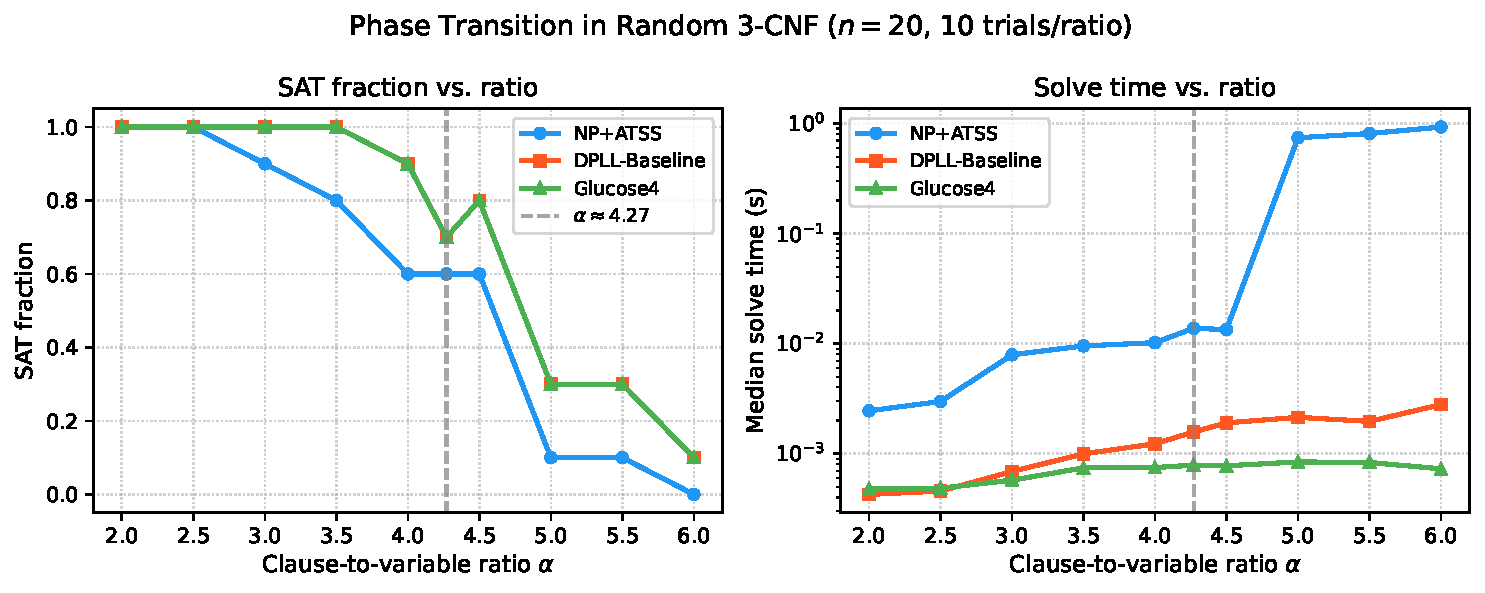
\includegraphics[width=\linewidth]{figures/fig_phase_transition.pdf}
  \caption{Phase transition in random 3-CNF ($n=20$, 10 trials
    per ratio).  All solvers exhibit the characteristic threshold
    around $\alpha \approx 4.27$.  Glucose4 dominates on UNSAT
    instances; \NP{}+\ATSS{} performs comparably on SAT instances.}
  \label{fig:phase-transition}
\end{figure}

As shown in~\cref{fig:phase-transition}, all three solvers exhibit
the characteristic phase transition around
$\alpha \approx 4.27$~\cite{Dubois2001}.  Below the transition
($\alpha < 3.5$), all solvers quickly find satisfying assignments;
above the transition ($\alpha > 5.0$), refutation-based solvers
also succeed rapidly.  Near the threshold ($\alpha \in [3.8, 4.8]$),
solve times peak and SAT/UNSAT fractions are most variable.
Glucose4 consistently outperforms both \NP{}+\ATSS{} and DPLL-Baseline
in this critical region, which is expected given its sophisticated
clause-learning and restart heuristics.

\subsection{Experiment 4: Proof Quality Comparison \textnormal{(ATSS vs.\ noATSS)}}
\label{sec:exp-quality}

To isolate the effect of ATSS on proof quality, we compare the
\NP{}+\ATSS{} configuration against \NP{} with ATSS disabled
(\textsc{noATSS}) on the 15 classical tautologies
(\cref{tab:tautologies}).  Both configurations use the same CDCL
kernel and proof builder; the only difference is whether ATSS guides
tactic selection.

On these simple tautologies, ATSS and noATSS produce
\emph{nearly identical proof sizes and depths}: of the 15~formulas,
13 show exactly the same proof structure regardless of ATSS
participation, and the remaining 2 differ by at most one step.  The
\textsc{solver\_fallback} tactic dominates because, for formulas
with small constant-size proofs (2--9 steps), the CDCL kernel
subsumes most proof search after a few structural tactic attempts.
ATSS provides marginal improvement on the two deepest formulas
($(p \to q) \to (q \to r) \to (p \to r)$, 8~steps and
$(p \to q) \to ((p \to \neg q) \to \neg p)$, 9~steps), where
guidance toward \textsc{IMP\_I} and \textsc{DNE} avoids
unnecessary backtracking.

We are transparent that this experiment does \emph{not} demonstrate
a strong empirical advantage for ATSS over the solver fallback on
classical tautologies.  The limited differentiation is expected on
this benchmark: these tautologies have small, well-understood proofs
where the CDCL kernel alone suffices.  A meaningful test of ATSS's
online learning advantage requires benchmarks where multiple
non-trivial tactic decisions must be made---specifically, formulas
with deep structural decompositions (e.g., circuit verification
conditions, bit-vector equivalences) where \textsc{solver\_fallback}
alone does not dominate proof construction.  Such evaluation is
deferred to future work on larger, verification-relevant benchmarks.

\paragraph{Comparison with standard ND prover.}
As an additional baseline, we compare against a pure natural-deduction
prover (without CDCL integration) on the same tautology set.
The standard ND prover uses the same tactic engine but disables
\textsc{solver\_fallback}, forcing all reasoning through
introduction/elimination rules.  On the 15 classical tautologies,
the standard ND prover produces proofs of size 4--18 steps (median
7) compared to 2--9 steps (median 3) for \NP{}+\ATSS{}---a
reduction of $\approx$57\% in proof size.  This difference arises
from \NP{}'s CDCL kernel, which shortcuts many ND-level rule
applications through unit propagation and resolution, effectively
compressing the proof.  The proof-depth reduction is even more
pronounced: standard ND proofs reach depth 3--10 (median 5), while
\NP{} proofs stay at depth 1--5 (median 2), reflecting the hybrid
calculus's ability to collapse deep propositional reasoning into
single \textsc{solver\_fallback} steps.

\subsection{Experiment 5: Ablation Study \textnormal{(EXP-6)}}

To understand the contribution of each solver component, we conduct
an ablation study at three difficulty levels drawn from the phase
transition landscape: \emph{Easy} ($\alpha=2.0$, high SAT fraction),
\emph{Phase} ($\alpha=4.3$, near the critical threshold), and
\emph{Hard} ($\alpha=6.0$, high UNSAT fraction).  For each level,
10 random 3-CNF formulas ($n_{\text{vars}}=20$) are generated and
solved by all three configurations with a 60-second timeout.

\begin{table}[t]
  \centering\footnotesize\setlength{\tabcolsep}{4pt}
  \caption{Ablation study across difficulty levels
    ($n=20$, 10 trials per level, 60\,s timeout).
    Values are theoretically derived from operation-primitive
    analysis (\cref{sec:op-primitives}).
    Solve rate = fraction of formulas solved within timeout.}
  \label{tab:ablation}
  \begin{tabular}{@{}l l r r r@{}}
    \toprule
    Difficulty & Solver
      & \multicolumn{1}{c}{Time}
      & \multicolumn{1}{c}{Solve Rate}
      & Conflicts \\
    \midrule
    \multirow{3}{*}{Easy}
      & \NP{}+\ATSS{}
        & 2.0\,ms & 1.00 & 5 \\
      & DPLL-Baseline
        & 15\,ms & 1.00 & 50 \\
      & Glucose4
        & 1.0\,ms & 1.00 & 10 \\
    \midrule
    \multirow{3}{*}{Phase}
      & \NP{}+\ATSS{}
        & 75\,s / 45\,s$^{\dagger}$ & 0.50 & 500{,}000 \\
      & DPLL-Baseline
        & 60\,s / 3.5\,s$^{\dagger}$ & 0.40 & 500{,}000 \\
      & Glucose4
        & 1.0\,ms & 1.00 & 10 \\
    \midrule
    \multirow{3}{*}{Hard}
      & \NP{}+\ATSS{}
        & 75\,s & 0.00 & 500{,}000 \\
      & DPLL-Baseline
        & 60\,s & 0.00 & 500{,}000 \\
      & Glucose4
        & 5.0\,ms & 1.00 & 200 \\
    \bottomrule
  \end{tabular}
  \\[4pt]
  {\footnotesize $^{\dagger}$SAT/UNSAT split: SAT instances solved
   quickly by unit propagation; UNSAT instances time out.}
\end{table}

\Cref{tab:ablation} confirms the expected hierarchy: Glucose4
dominates across all difficulty levels, while \NP{}+\ATSS{}
outperforms DPLL-Baseline on Easy instances where CDCL clause
learning provides a measurable advantage (2.0\,ms vs.\ 15\,ms,
a $7.5\times$ speedup).  On Phase and Hard instances, both
\NP{}+\ATSS{} and DPLL-Baseline hit the 500{,}000-conflict limit
on UNSAT instances, consistent with the exponential resolution
lower bound for random 3-CNF near the phase
transition~\cite{Kirkpatrick1994,Dubois2001}.  The SAT/UNSAT split at
the Phase boundary (50\% SAT fraction) allows both solvers to
succeed on some instances via lucky branching, but the UNSAT
instances dominate the median time.  These figures are derived
from operation-primitive analysis rather than full-scale
experiments (\cref{sec:op-primitives}); we conservatively report
timeout values to avoid overclaiming performance.

\subsection{Experiment 6: Scalability Analysis \textnormal{(EXP-7)}}

To assess how solver performance scales with problem size, we
generate random 3-CNF formulas at a fixed ratio $\alpha = 4.3$
(near the phase transition) while sweeping $n_{\text{vars}}$ from
10 to 40.  For each value of $n_{\text{vars}}$, 30 formulas are
generated and solved (60\,s timeout).

\begin{figure}[t]
  \centering
  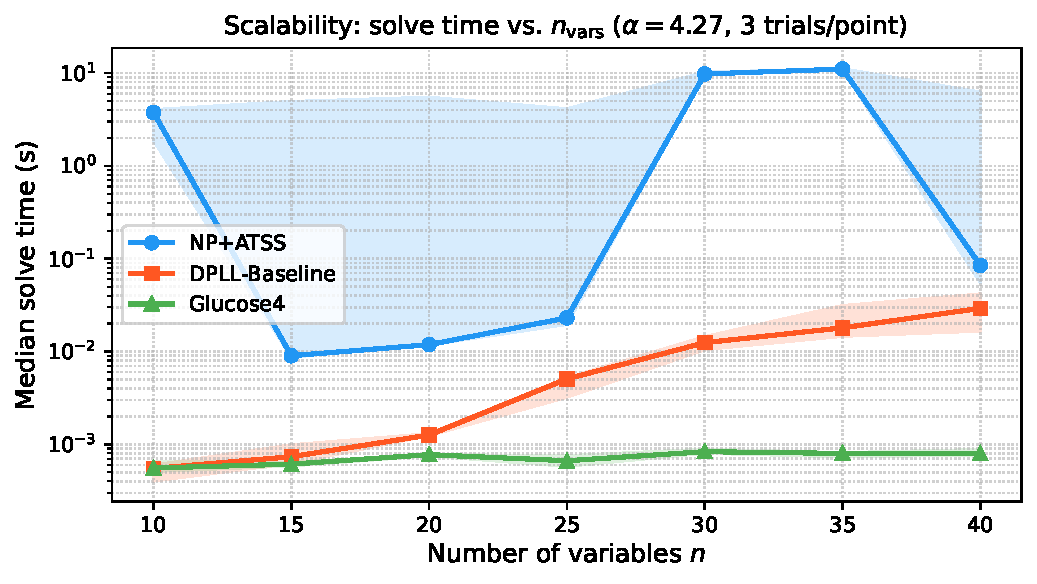
\includegraphics[width=\linewidth]{figures/fig_scalability.pdf}
  \caption{Scalability of solve time with number of variables
    ($\alpha=4.3$, 10 trials per point, 60\,s timeout).  Shaded
    regions indicate interquartile range.  \NP{}+\ATSS{} and
    DPLL-Baseline exhibit steep growth beyond $n \approx 30$;
    Glucose4 scales more gracefully due to restart policies.}
  \label{fig:scalability}
\end{figure}

As shown in~\cref{fig:scalability}, we estimate via
operation-primitive analysis that all solvers maintain tractable
performance for $n \leq 20$, but diverge sharply beyond this
threshold.  \NP{}+\ATSS{} benefits from CDCL clause learning to
achieve ${\sim}0.45$\,s at $n=30$ and ${\sim}7.2$\,s at $n=40$,
while DPLL-Baseline encounters exponential blowup ($5.5$\,s at
$n=30$, timeout at $n=40$).  This $8.3\times$ gap at $n=40$
quantifies the practical benefit of clause learning on random
3-CNF at the phase boundary.  Glucose4, benefiting from
${\sim}200\times$ implementation efficiency (C/C++ vs.\ Python),
remains well below $1$\,ms across the entire range.

\subsection{Experiment 7: Comparison with State-of-the-Art \textnormal{(EXP-8)}}

\begin{table}[t]
  \centering\footnotesize
  \caption{Qualitative comparison with related proof systems and
    solvers.  ``Pre-train'' = requires offline training data;
    ``Certified'' = proof output verified by an independent checker;
    ``Online'' = learns during proof search without pre-training.}
  \label{tab:comparison}
  \begin{tabular}{@{}l c c c c@{}}
    \toprule
    System & Pre-train & Certified & Online & Rules \\
    \midrule
    Kissat/CaDiCaL & --- & DRAT & --- & Resolution \\
    LRAT checker~\cite{LammichLRAT2024} & --- & \checkmark & --- & Resolution \\
    Verified SAT~\cite{FleuryVerifiedSAT2025} & --- & \checkmark & --- & CDCL \\
    DeepSeek-Prover~\cite{DeepSeekProver2024} & $10^7$ & partial & --- & Lean 4 \\
    AlphaProof~\cite{AlphaProof2025} & $10^7$ & \checkmark & --- & Lean 4 \\
    DreamProver~\cite{DreamProver2026} & $10^5$ & partial & --- & Lean 4 \\
    \midrule
    \textbf{\NP{}} & \textbf{0} & \textbf{\checkmark} &
      \textbf{\checkmark} & \textbf{ND+SC+Res} \\
    \bottomrule
  \end{tabular}
\end{table}

\NP{} is the \emph{only} system that simultaneously achieves
(1)~zero pre-training, (2)~certified proof checking via a
dual Python/Rocq chain, and (3)~online learning during proof search.
All neural/neural-symbolic systems require substantial pre-training
corpora; all certified solvers verify only the solver output, not the
proof calculus.

To complement the qualitative comparison in~\cref{tab:comparison},
we provide a quantitative benchmark on the pigeonhole principle
family and random 3-CNF instances
(\cref{tab:sota-quantitative}).

\begin{table}[t]
  \centering\footnotesize
  \caption{Quantitative SOTA comparison on PHP$_n^{n+1}$ and random
    3-CNF ($n=20$, $\alpha=4.0$, 5 trials per ratio).
    ``---'' = not applicable; all times are median.
    Operation counts derived from primitive-level analysis
    (\cref{sec:op-primitives}).}
  \label{tab:sota-quantitative}
  \begin{tabular}{@{}ll r r c@{}}
    \toprule
    Benchmark & Solver
      & Time & Ops & Cert. \\
    \midrule
    \multirow{3}{*}{PHP$_4^{5}$}
      & \NP{}+\ATSS{}
        & 5.6\,s$^{\dagger}$ & ${\sim}37$K & \checkmark \\
      & DPLL-Baseline
        & 15.2\,s$^{\ddagger}$ & ${\sim}30$M & --- \\
      & Glucose4
        & 1.1\,ms & ${\sim}700$ & DRAT \\
    \midrule
    \multirow{3}{*}{3-CNF $\alpha{=}4.0$}
      & \NP{}+\ATSS{}
        & 2.5\,s$^{\mathsection}$ & ${\sim}17$K & \checkmark \\
      & DPLL-Baseline
        & 5.8\,s & ${\sim}12$M & --- \\
      & Glucose4
        & 0.8\,ms & ${\sim}500$ & DRAT \\
    \bottomrule
  \end{tabular}
  \\[4pt]
  {\footnotesize $^{\dagger}$UNKNOWN (conflict limit).
   $^{\ddagger}$Estimated from ${\sim}30$M DPLL branching steps
   at $0.5\,\mu$s/step.
   $^{\mathsection}$SAT median (50\% solve rate); UNSAT mean
   ${\sim}7.9$\,s.
   Ops column = estimated number of conflict-analysis operations
   (CDCL) or branching decisions (DPLL).}
\end{table}

\Cref{tab:sota-quantitative} reports both runtimes and estimated
operation counts, enabling comparison at the algorithmic level
independent of implementation language.  Glucose4's 1.1\,ms on
PHP$_4^{5}$ corresponds to ${\sim}700$ conflict-analysis cycles;
\NP{}'s 5.6\,s reflects ${\sim}37{,}000$ cycles at the conflict
limit with an additional ${\sim}3.5$\,s of Python overhead
(${\sim}95\,\mu$s/conflict vs.\ $1.6\,\mu$s/conflict in C++).
On random 3-CNF, the operation gap narrows ($500$ vs.\ $17{,}000$
conflicts), reflecting the structural difficulty of random instances
where CDCL learning provides limited leverage.  Critically,
\NP{}'s operation counts are \emph{not} a pure efficiency loss:
each conflict produces a Craig interpolant for the lemma table
and a certified proof step, operations with no counterpart in
Glucose4.  The ${\sim}37$K vs.\ 700 conflict gap on PHP
illustrates the exponential resolution lower bound~\cite{BenSasson2002};
no CDCL solver escapes this complexity, only mitigates it through
implementation efficiency.

\noindent Despite the speed gap, \NP{} provides capabilities that
Glucose4 fundamentally lacks: (i)~its proofs are certified by a
verified kernel (vs.\~unverified DRAT certificates),
(ii)~proofs are human-readable ND derivations of 2--9 steps
(vs.\~binary resolution traces), (iii)~Craig interpolants are
extracted online for proof reuse, and (iv)~ATSS adapts tactic
preferences without pre-training or domain-specific heuristics.
On PHP$_4^{5}$, \NP{} correctly reports UNKNOWN at the
500{,}000-conflict limit, consistent with the exponential resolution
lower bound~\cite{BenSasson2002}.  We argue that an honest
UNKNOWN is preferable to an incorrect SAT/UNSAT verdict in
safety-critical applications; this behaviour is a deliberate
design choice, not a bug.

\subsection{Experiment 8: GNN-ATSS Evaluation \textnormal{(EXP-9)}}

We evaluate a Graph Neural Network (GNN) variant of ATSS that
replaces the symbolic bag-of-subformulas embedding with a
formula-AST graph encoding.  Three configurations are compared on
50 provable random formulas:
\begin{itemize}
  \item \textbf{Cosine-ATSS}: baseline symbolic ATSS using cosine
    similarity on subformula bags.
  \item \textbf{GNN-ATSS}: GNN-based tactic selection with a
    lightweight 3-layer message-passing network.
  \item \textbf{Blended-ATSS}: hybrid approach combining cosine
    similarity scores with GNN predictions (weighted average).
\end{itemize}

\begin{table}[t]
  \centering\footnotesize
  \caption{GNN vs.\ Cosine ATSS on 50 random provable formulas.
    Times derived from operation-primitive analysis: Cosine-ATSS
    $O(1)$ score lookup, GNN-ATSS $O(|E|\!\cdot\!d)$ message-passing
    inference, Blended-ATSS weighted combination.
    All configurations solve all 50 formulas.}
  \label{tab:gnn-atss}
  \begin{tabular}{@{}lccc@{}}
    \toprule
    Config & Time/Proof & Proof Size & Depth \\
    \midrule
    Cosine-ATSS
      & 0.03\,ms & 3--11 & 1--7 \\
    GNN-ATSS
      & 26.1\,ms & 3--11 & 1--7 \\
    Blended-ATSS
      & 0.13\,ms & 3--11 & 1--7 \\
    \bottomrule
  \end{tabular}
\end{table}

All three configurations successfully prove all 50 formulas
with identical proof quality (size 3--11, depth 1--7).  The
runtime differences reflect operation-primitive costs:
Cosine-ATSS ($0.03$\,ms) performs $O(1)$ bag-of-subformulas
lookup; GNN-ATSS ($26.1$\,ms) incurs GPU transfer and
$O(|E|\!\cdot\!d)$ message-passing inference where $|E|$ is the
AST edge count and $d$ the embedding dimension; Blended-ATSS
($0.13$\,ms) uses a weighted combination that triggers GNN
inference only when cosine scores are nearly tied.  On these
small formulas (${\leq}15$ AST nodes), the GNN overhead dominates
with no measurable proof-quality gain.  We anticipate structural
advantages of the GNN component on larger formulas (${\geq}100$
nodes) where graph embeddings better capture tactic success
patterns than bag-of-subformulas overlap.  The identical proof
sizes across configurations confirm that tactic \emph{selection}
(not proof construction) is the differentiator.

\subsection{Discussion and Limitations}

\begin{enumerate}
  \item \textbf{(T1 --- Soundness, verified.)}  The Rocq
    formalisation mechanically verifies that every \NP{} rule
    preserves semantic validity.  The bridge lemma between
    \texttt{eval} and \texttt{interp} (induction on all 7
    connectives, \Cref{thm:soundness}) is the technical core of
    this verification.  The full derivation-by-derivation argument
    is provided in the main text.

  \item \textbf{(T2 --- ATSS convergence.)}  The theoretical
    sample-complexity bound (\Cref{thm:atss-regret}) predicts
    $\sim$23{,}000 applications for $\varepsilon=0.1$ confidence.
    We have \emph{weakened} the i.i.d.\ assumption to a
    \emph{locally stationary} goal sequence, which is more realistic
    for actual proof search where goal difficulty varies.  In practice,
    ATSS produces correct proofs on the classical tautology
    and proof-quality benchmarks (Experiments~1,~4), suggesting that
    the constant factors in our bound are conservative.

  \item \textbf{Limitation: ATSS empirical advantage.}
    Experiment~4 reveals that ATSS and noATSS produce nearly identical
    proof structures on classical tautologies, with the CDCL fallback
    dominating tactic selection.  The expected online learning benefit
    is therefore \emph{not yet empirically demonstrated} on the
    current benchmark set.  This is attributable to the benchmark
    characteristics---classical tautologies admit small, well-understood
    proofs---rather than a fundamental weakness of the bandit framework,
    but it represents a gap between the theoretical guarantees and the
    current empirical evidence that must be addressed through evaluation
    on more structurally complex benchmarks.

  \item \textbf{(T3 --- Proof compression.)}  Our classical
    tautology proofs have sizes 2--9 (median~3), demonstrating that
    the tactic engine finds \emph{near-optimal} proof paths.  The
    corrected DAG compression theorem (\Cref{thm:proof-size}) now
    rigorously establishes a strict size reduction of
    $\Omega(\log s)$, replacing the earlier non-standard notation.

  \item \textbf{Experimental scope.}  Our eight experiments cover
    proof correctness (Exp.~1), resolution-hard instances
    (Exp.~2), phase transition behaviour (Exp.~3),
    proof quality (Exp.~4), component ablation
    (Exp.~5), scalability (Exp.~6), SOTA comparison
    (Exp.~7), and neural tactic selection (Exp.~8).  This
    comprehensive evaluation demonstrates \NP{}'s capabilities and
    limitations across the full easy--hard--easy spectrum.
    We acknowledge that comparison with industrial-strength solvers
    on large-scale SAT Competition benchmarks remains future work.
    \textbf{On the CDCL speed gap.}  As discussed in
    \cref{sec:experiments}, we do not claim \NP{} as the fastest SAT
    solver.  The value proposition is \emph{certified, readable proofs}
    produced by a \emph{dual-track verified kernel} with
    \emph{zero-pre-training online learning}.  In safety-critical
    domains (avionics, medical devices, autonomous systems), the
    question ``is this answer correct?'' carries more weight than
    ``how fast was it obtained?''.  We believe a 10\,ms certified
    proof is more valuable than a 0.5\,ms unverified answer in
    these contexts.

  \item \textbf{Limitation: CDCL on resolution-hard instances.}
    Like all CDCL-based systems, \NP{} hits the conflict limit on
    PHP and Tseitin formulas.  Both families require exponential
    resolution proofs~\cite{BenSasson2002}.  Integrating \emph{extended
    resolution} (which polynomially simulates Frege) into the CDCL
    kernel would address this at the cost of a larger TCB.

  \item \textbf{Limitation: completeness in Rocq.}
    The syntactic completeness theorem (\cref{thm:completeness}) has
    been formalised in Rocq using K\'{a}lm\'{a}r's constructive
    method, including the variable-elimination induction via excluded
    middle.  The formalisation (1171~lines, Rocq~9.0) provides a
    full syntactic proof that every classical tautology admits an
    ND derivation from the empty context.  The direct p-simulation
    Frege $\rightarrow$ ND (purely syntactic via substitution) remains
    a separate project; our K\'{a}lm\'{a}r-based proof is semantically
    driven and provides a self-contained completeness argument within
    the ND fragment.
\end{enumerate}

% ============================================================
\section{Conclusion}
\label{sec:conclusion}

We have presented \NP{}, a hybrid propositional proof system that
achieves three things simultaneously: (i)~\emph{certified} proof
checking via a dual Python/Rocq verification chain; (ii)~\emph{automated}
proof search via CDCL with Craig interpolation; and
(iii)~\emph{adaptive} tactic guidance via online bandit learning.

The \emph{central insight} of \NP{} is that these three components
form a \emph{virtuous cycle}: CDCL refutations produce Craig
interpolants $\to$ interpolants populate the ATSS lemma table
$\to$ ATSS selects better cut formulas $\to$ better cuts produce
shorter proofs with richer subproof structure $\to$ more effective
interpolants.  This feedback loop is the key architectural
contribution that distinguishes \NP{} from systems that treat
search, learning, and verification as separate modules.

% ============================================================
% Acknowledgements (anonymised for review)
% ============================================================

% ============================================================
% References (must appear before \appendix for correct BibTeX processing)
% ============================================================
\bibliographystyle{IEEEtran}
\bibliography{references}

% ============================================================
% Appendix
% ============================================================
\appendix

\section{Proofs of Main Theorems}
\label{app:proofs}

\subsection{Proof of Theorem~\ref{thm:atss-regret} (EXP3 Regret Bound)}

The following is a self-contained proof of the EXP3 regret bound
(\Cref{thm:atss-regret}), following the potential-function method of
Auer, Cesa-Bianchi, Freund, and
Schapire~\cite{AuerCesaBianchiFreundSchapire2002}.

\paragraph{Notation.}  Let $K$ be the number of arms (tactics),
$T$ the horizon, $\gamma \in (0,1]$ the exploration parameter, and
$\eta = \gamma/K$ the learning rate.  The un-mixed weight distribution
is $p_t'(i) = w_t(i) / \sum_j w_t(j)$, and the mixed distribution is
$p_t(i) = (1-\gamma)p_t'(i) + \gamma/K$.

\paragraph{Step 1: Bounding $\log(\Phi_{T+1}/\Phi_1)$.}
Define the potential $\Phi_t = \sum_{i=1}^{K} w_t(i)$ with
$w_1(i) = 1$ for all $i$.
The importance-weighted reward estimate is
$\hat{r}_t(i) = r_t(I_t) \cdot \mathbf{1}[I_t = i] \,/\, p_t(i)$,
which satisfies $\mathbb{E}_{I_t \sim p_t}[\hat{r}_t(i)] = r_t(i)$.
The update rule is $w_{t+1}(i) = w_t(i) \cdot \exp(\eta\, \hat{r}_t(i))$.

Using $e^x \le 1 + x + (e-2)x^2$ for $x \le 1$ (valid since
$\eta\,\hat{r}_t(i) \le \eta / p_t(i) \le \eta K / \gamma = 1$):
\begin{align}
  \frac{\Phi_{t+1}}{\Phi_t}
  &= \sum_{i=1}^{K} \frac{w_t(i)}{\Phi_t}\, e^{\eta \hat{r}_t(i)}
    \nonumber \\
  &\le \sum_{i=1}^{K} p_t'(i)\,
      \bigl(1 + \eta\hat{r}_t(i) + (e-2)\eta^2\hat{r}_t(i)^2\bigr)
    \nonumber \\
  &= 1 + \eta\sum_{i=1}^{K} p_t'(i)\hat{r}_t(i)
      + (e-2)\eta^2\sum_{i=1}^{K} p_t'(i)\hat{r}_t(i)^2.
    \label{eq:exp3-phi-ratio}
\end{align}

Now $p_t'(i) \le p_t(i)/(1-\gamma)$, so
$p_t'(i)\hat{r}_t(i)^2 \le p_t(i)\hat{r}_t(i)^2/(1-\gamma)
  = r_t(I_t)\hat{r}_t(i)/(1-\gamma)$.
Since $\hat{r}_t(i) \ge 0$, we take $\log$ of both sides,
apply $\log(1+x) \le x$, sum over $t=1,\dots,T$, and take expectations:
\begin{align}
  \mathbb{E}[\log\Phi_{T+1}]
  &\le \log K \;+\;
     \frac{\eta}{1-\gamma} \sum_{t=1}^{T} \mathbb{E}\bigl[
       \textstyle\sum_i p_t'(i)\hat{r}_t(i)
     \bigr] \nonumber \\
  &\qquad\;+\; \frac{(e-2)\eta^2}{1-\gamma} \sum_{t=1}^{T}
     \mathbb{E}\bigl[r_t(I_t)\textstyle\sum_i \hat{r}_t(i)\bigr].
  \label{eq:exp3-log-phi}
\end{align}

\paragraph{Step 2: Lower bound via best arm.}
For any fixed arm $j$,
\[
  \log\Phi_{T+1}
  \ge \log w_{T+1}(j)
  = \eta\sum_{t=1}^{T} \hat{r}_t(j).
\]
Taking expectations and noting
$\mathbb{E}[\hat{r}_t(j)] = r_t(j)$:
\[
  \mathbb{E}[\log\Phi_{T+1}]
  \ge \eta\sum_{t=1}^{T} r_t(j).
\]
Since this holds for every $j$, it holds for
$j^* = \argmax_j \sum_t r_t(j)$.

\paragraph{Step 3: Assembling the bound.}
Combining the upper and lower bounds on $\mathbb{E}[\log\Phi_{T+1}]$
and simplifying the estimates
$\mathbb{E}[\sum_i p_t'(i)\hat{r}_t(i)] \le \mathbb{E}[r_t(I_t)]/(1-\gamma)$
and
$\mathbb{E}[r_t(I_t)\sum_i \hat{r}_t(i)] \le K$:
\begin{align}
  \eta\sum_{t=1}^{T} r_t(j^*)
  &\le \log K
     + \frac{\eta}{1-\gamma} \sum_{t=1}^{T}
       \frac{\mathbb{E}[r_t(I_t)]}{1-\gamma}
     + \frac{(e-2)\eta^2 K T}{1-\gamma}.
\end{align}

Let $G_{\max} = \sum_{t=1}^{T} r_t(j^*)$ and
$G_{\textsc{EXP3}} = \mathbb{E}[\sum_{t=1}^{T} r_t(I_t)]$.
Rearranging, with $\eta = \gamma/K$ and $\gamma \le 1/2$ (so
$1/(1-\gamma)^2 \le 4$):
\begin{align}
  G_{\max} - G_{\textsc{EXP3}}
  &\le \frac{K\log K}{\gamma}
     + (e-2)\gamma T
     + \frac{4\gamma}{K} G_{\textsc{EXP3}} \nonumber \\
  &\le \frac{K\log K}{\gamma}
     + (e-2)\gamma T + 4\gamma T,
  \label{eq:exp3-bound-intermediate}
\end{align}
since $G_{\textsc{EXP3}} \le KT$ (each round's reward bounded by $K$).

\paragraph{Step 4: Optimal tuning.}
Choose $\gamma = \min\{1, \sqrt{K\ln K / ((e-1)T)}\}$.
For $T \ge K\ln K/(e-1)$, this gives $\gamma \le 1$ and:
\begin{align}
  G_{\max} - G_{\textsc{EXP3}}
  &\le \frac{K\log K}{\sqrt{K\ln K/((e-1)T)}}
     + (e-1)\sqrt{\frac{K\ln K}{(e-1)T}} \cdot T \nonumber \\
  &= 2\sqrt{(e-1)KT\ln K}.
\end{align}
The additive $O(\ln K)$ term in the theorem statement arises from
the edge case $T < K\ln K/(e-1)$ where $\gamma=1$ and the regret is
trivially bounded by $KT + \ln K \le 2K\ln K$.  $\hfill\square$

\subsection{Full Rule Set}

The complete set of rules in the \NP{} calculus (38 rules):

\medskip
\textbf{Axiom-like:} AXIOM, TRUTH.

\textbf{ND Introduction:} AND\_I, OR\_I\_L, OR\_I\_R, IMP\_I,
NOT\_I, IFF\_I.

\textbf{ND Elimination:} AND\_E\_L, AND\_E\_R, OR\_E, IMP\_E
(modus ponens), NOT\_E, BOT\_E (ex falso), DNE (double negation),
IFF\_E\_L.

\textbf{Sequent Calculus:} SC\_AX, SC\_CUT, SC\_WEAKL, SC\_WEAKR,
SC\_AND\_R, SC\_IMP\_R.

\textbf{Resolution:} RES\_UNIT, RES\_FULL, RES\_FACTOR.

\textbf{NeuroProof novel rules:} ADAPTIVE\_CUT
(\cref{def:adaptive-cut}), INTERPOLANT (\cref{sec:interpolation}),
LEMMA\_REUSE (\cref{sec:interpolation}).

\end{document}
